\documentclass[11pt]{article}
\usepackage[sc]{mathpazo} %Like Palatino with extensive math support
\usepackage{fullpage}
\usepackage[authoryear,sectionbib,sort]{natbib}
\linespread{1.7}
\usepackage[utf8]{inputenc}
\usepackage{lineno}


%%%%%%%%%%%%%%%%%%%%%
% LaTeX packages
%%%%%%%%%%%%%%%%%%%%%
% Please be sparing in your use of additional LaTeX packages, and
% upload any required style files to Editorial Manager with the file
% type "LaTeX ancillary files (.sty, .bst)."
\usepackage{gensymb}
\usepackage{booktabs}
\usepackage{multirow}
\usepackage{graphicx}
\usepackage{natbib}
\usepackage{rotating}
\usepackage{hyperref}
\usepackage{setspace} % remove this if submitting to Am. Nat., because the line spacing for figure and tables should be double spaced.
\renewcommand{\arraystretch}{1.3} % likely need to remove if submitting to Am. Nat.


%%%%%%%%%%%%%%%%%%%%%
% Line numbering
%%%%%%%%%%%%%%%%%%%%%
\usepackage{lineno}
% Please use line numbering with your initial submission and
% subsequent revisions. After acceptance, please comment out 
% the commands \usepackage{lineno}, \linenumbers{} 
% and \modulolinenumbers[3] below.

%%%%%%%%%%%%%%%%%%%%%
% File path for figures
%%%%%%%%%%%%%%%%%%%%%
% Depends on 'graphicx' package
\graphicspath{ {figures/} }

\title{Host-plant genetic variation dominates phenotypic plasticity in structuring above and belowground communities}

%%%%%%%%%%%%%%%%%%%%%
% Authorship
%%%%%%%%%%%%%%%%%%%%%
% Please remove authorship information while your paper is under review,
% unless you wish to waive your anonymity under double-blind review. 
% Remember to uncomment the information after acceptance.

\author{Matthew A. Barbour$^{1,\ast}$ \\ 
Generic H. Collaborator$^{2,\dag}$ \\ 
Additional Q. Expert$^{3,\ddag}$}

\date{}

\begin{document}

\maketitle

\noindent{}1. University of Chicago, Chicago, Illinois 60637;

\noindent{}2. University of Toronto, Toronto, Ontario M5S 1A5, Canada;

\noindent{}3. Middle Eastern Technical University, \c{C}ankaya, 
Ankara 06800, Turkey.

\noindent{}$\ast$ Corresponding author; e-mail: matthew.barbour@ieu.uzh.ch.

\noindent{}$\ddag$ ORCIDs: Cook, 0000-0002-1234-5678; Collaborator, 0000-0001-5678-9123; Expert, 0000-0003-3456-789X.

\bigskip

\textit{Manuscript elements}: Figure~1, figure~2, table~1, online
appendices~A and B (including figure~A1 and figure~A2). Figure~2 is to
print in color.

\bigskip

\textit{Keywords}: Examples, model, template, guidelines.

\bigskip

\textit{Manuscript type}: Article. 
% Or e-article, note, e-note, natural history miscellany,
% e-natural history miscellany, comment, reply, symposium, or
% countdown to 150.

\bigskip

\noindent{\footnotesize Prepared using the suggested \LaTeX{} 
template for \textit{Am.\ Nat.}}

\linenumbers{}
\modulolinenumbers[3]

\newpage{}

\section*{Abstract}
\begin{enumerate}
\item
  Host-plant genetic variation affects the diversity and composition of
  associated above and belowground communities. Most evidence supporting
  this view is derived from studies within a single common garden,
  thereby constraining the range of biotic and abiotic environmental
  conditions that might directly or indirectly (via phenotypic
  plasticity) affect communities. If natural variability in the
  environment renders host-plant genetic effects on associated
  communities unimportant, then studying the community-level
  consequences of genetic variation may not be warranted.
\item
  We addressed this knowledge gap by planting a series of common gardens
  consisting of 10 different clones (genotypes) of the willow
  \emph{Salix hookeriana} in a coastal dune ecosystem and manipulated
  natural variation in ant-aphid interactions (biotic) and wind exposure
  (abiotic) in two separate experiments. We then quantified the
  responses of associated species assemblages both above (foliar
  arthropods) and belowground (rhizosphere fungi and bacteria). In
  addition, we quantified plant phenotypic responses (plant growth, leaf
  quality, and root quality) to tease apart the effects of heritable
  trait variation, phenotypic plasticity, and direct environmental
  effects on associated communities.
\item
  In the ant-aphid experiment, we found that willow genotype explained
  more variation in foliar arthropod communities than aphid additions
  and proximity to aphid-tending ant mounds. However, aphid additions
  modified willow genotype effects on arthropod community composition by
  attracting other aphid species to certain willow genotypes. In the
  wind experiment, wind exposure explained more variation than willow
  genotype in communities of foliar arthropods and root bacteria. Still,
  willow genotype had strong effect sizes on several community
  properties of arthropods and fungi, indicating that host-plant genetic
  variation remains important. In both experiments, plant-growth traits
  were the primary determinants of arthropod community structure with
  leaf quality traits playing a lesser role; however, we failed to
  identify which root traits were mediating belowground community
  responses.
\item
  Taken together, our results suggest that host-plant genetic variation
  is an important driver of above and belowground biodiversity, despite
  natural variation in the biotic and abiotic environment.
\end{enumerate}

\newpage{}

\section*{Introduction}

% The journal does not have numbered sections in the main portion of
% articles. Please refrain from using section references such as
% section~\ref{section:CountingOwlEggs}, and refer to sections by name
% (e.g. section ``Counting Owl Eggs'').

Intraspecific genetic variation is a key driver of trait variation
within host plants, which in turn can have cascading effects on
associated species and entire communities of organisms
\cite{Fritz_1988}\cite{Lamit_2016}\cite{Maddox_1990}\cite{antonovics1992toward}. For
example, genetic variation in the leaf chemistry of cottonwoods
\cite{Whitham_2006} and in the plant architecture of coyote bush
\cite{Crutsinger_2014} structures diverse assemblages of species, from foliar
arthropods aboveground to soil microbes below. While community-level
consequences of genetic variation (commonly referred to as `community
genetics', sensu~\cite{antonovics1992toward}) have been documented in a variety of
host-plant taxa \cite{Whitham_2012}, evidence comes primarily from common
garden experiments that minimize environmental variation. These
controlled environments likely limit effects of the biotic and abiotic
environment on the expression of host plant traits \cite{Gratani_2014} as
well as the diversity and composition of species assemblages
\cite{macarthur1972geographical}\cite{Gaston_2000}. Therefore, the importance of
host-plant genetic variation in structuring ecological communities in
naturally varying environments remains unclear
\cite{Hersch_Green_2011}\cite{Tack_2011}\cite{Crutsinger_2015}.

A key challenge for advancing studies of community genetics beyond the
common garden is to identify important biotic and abiotic environmental
factors that structure communities associated with host plants. For
example, a series of experiments in common milkweed (\emph{Asclepias
syriaca}) have shown that a diversity of biotic factors, such as light
competition from neighboring plants \cite{Agrawal_2003}, caterpillar
herbivory \cite{Abdala_Roberts_2012}, and aphid-tending
ants~\cite{Mooney_2008}\cite{Abdala_Roberts_2012} can act independently or interact
with milkweed genotype to shape its associated community of foliar
arthropods. Similarly, abiotic factors, such as soil nutrient
availability, can act independently or modify the effects of host-plant
genotype on herbivore assemblages \cite{Orians_1996} and tri-trophic
interactions \cite{Rossi_1998}\cite{Abdala_Roberts_2012a}. Still, we are lacking
explicit comparisons of host-plant genotypic effects across natural
gradients in both biotic and abiotic factors, so their relative
importance in structuring communities is unclear.

Although host plants provide essential resources for a diverse array of
taxa both above- and belowground, the majority of community genetics
studies have focused on aboveground assemblages \cite{Whitham_2012}.
Studies that have simultaneously examined above- and belowground
communities have found variable results, with host-plant genetic effects
on aboveground communities being stronger
\cite{Crutsinger_2008}\cite{Bailey_2009} or comparable and coupled
\cite{Crutsinger_2014} with those belowground. Above- and belowground
linkages can have important consequences for both plant fitness
\cite{Whitham_2006} and terrestrial ecosystem processes \cite{Wardle_2004}.
In addition, feedbacks between above- and belowground assemblages may
depend strongly on the biotic and/or abiotic environment
\cite{Wardle_2004}. Consequently, a rising challenge for community
genetics is to understand the linkages between above- and belowground
communities \cite{Crutsinger_2014}\cite{Lamit_2015} and whether these
linkages are modified by environmental variation.

Host-plant traits determine the quantity and quality of resources for
the diverse organisms that colonize them; therefore, measuring
functional trait responses of host-plant genotypes to different
environments can give insight to mechanisms of community assembly in
genotype-by-environment studies. Phenotypic traits can vary in their
plasticity (change in trait expression of a genotype in response to the
environment: \cite{Scheiner_1993}) and may even be plastic in response to
one environmental gradient but not another
\cite{Scheiner_1993}\cite{Scheiner_1984}\cite{Garbutt_1987}. In addition,
multiple plant traits can be important in structuring associated
communities on host plants
\cite{Barbour_2015}\cite{Barbour_2016}\cite{Agrawal_2006}\cite{agrawal2005natural}\cite{Agrawal_2004}.
Simultaneous measurements of multiple functional traits and
community-level patterns in genotype-by-environment studies can
distinguish the effects of heritable trait variation (proportion of
variance in a trait explained by genotype: \cite{lynch1998genetics}),
phenotypic plasticity, and direct environmental effects on species
assemblages.

Here, we use common garden experiments to examine how host-plant
genotypic variation as well as the biotic and abiotic environment
structure communities associated with the willow \emph{Salix hookeriana}
in a coastal dune ecosystem. Prior work in this system has shown that
willow genotypes host distinct arthropod communities and that multiple
plant traits are important in determining community assembly
\cite{Barbour_2015}\cite{Barbour_2016}. Importantly, these traits varied
substantially in their degree of heritability (plant growth, mean
\(H^2\)= 0.26; leaf quality, mean \(H^2\) = 0.72),
suggesting that the environment may influence them in different ways. We
sought to answer the following questions: (1) What is the relative
importance of willow genotype vs. the biotic and abiotic environment in
structuring aboveground communities? (2) Do willow genetic and
environmental variation have different effects on above and belowground
communities? (3) What is the relative importance of genetic
variation, phenotypic plasticity, and direct environmental effects in
structuring communities?

% Please note that we prefer (\citealt{Xiao2015}) to \citep{Xiao2015},
% since \citep{} inserts a comma after "et al."

\section*{Methods}

\subsection*{Study site}

We conducted this research at Lanphere Dunes (40\
degree53'29.85''N,
124 degree symbol 8'49.06''W), a pristine coastal dune ecosystem managed by
US Fish and Wildlife service in Humboldt County, California, USA.
Coastal willow (\emph{Salix hookeriana} ex Barratt ex Hooker) naturally
occurs in nearshore dune swales -- seasonal freshwater wetlands that
form in depressions between dune ridges \cite{pickart2007beach}. Aside from
coastal willow (hereafter willow), the dominant vegetation in these
swales consists of beach pine (\emph{Pinus contorta} ssp.
\emph{contorta}) and slough sedge (\emph{Carex obnupta}).

During preliminary surveys, we qualitatively identified two important
sources of environmental variation for willows in the dunes -- one
biotic (the presence of ant-aphid mutualisms) and one abiotic (wind
exposure). We observed that the aphid \emph{Aphis farinosa} was an
abundant herbivore at Lanphere Dunes. \emph{Aphis farinosa} is usually
found at the tips of new shoot growth where it feeds on willow phloem.
As with many other aphid species, \emph{A. farinosa} excretes
carbohydrate-rich honeydew while feeding, which attracts ants that tend
the aphids and feed on the honeydew. This ant-aphid interaction is often
mutualistic, because the ants will defend aphids from predatory
arthropods and also eat other herbivores that may be competing with the
aphids \cite{Floate_1994}\cite{Mooney_2008}. The ant species we observed
most frequently tending \emph{A. farinosa} was the western thatching
ant, \emph{Formica obscuripes}. Western thatching ants create distinct
dome-shaped mounds from nearby plant-material and are known to reduce
herbivory from leaf chewing arthropods on \emph{S. hookeriana} at our
study site~\cite{CRUTSINGER_2005}, presumably by deterring ovipositing
females or predating young larva. This work suggests that the presence
of aphids and the proximity to ant mounds influences associated
communities through three non-mutually exclusive mechanisms: (i)
increased abundance of aphid-tending ants, which could deter other
arthropods; (ii) attraction of predators or deterrence of other
herbivores, by aphids; (iii) alteration of plant-growth or leaf quality
traits by aphids. We also observed that willows growing in wind-exposed
habitats often exhibit reduced growth, especially at their leading edge,
appearing to be ``swept back'' by the wind. We hypothesized that wind
exposure may influence associated communities through three non-mutually
exclusive mechanisms: (i) reduced plant size due to wind pruning; (ii)
altered soil characteristics due to increased evaporation; and (iii)
direct inhibition of ovipositing female arthropods.

\subsection*{Experimental design}

Prior to bud break in February 2012, we took shoot cuttings (40 cm
length \& \textasciitilde{}0.5 cm diameter) from one to two replicates
of 10 different willow genotypes from a pool of 26 locally collected
willow genotypes planted in a large common garden experiment. Details
about the establishment of this common garden are given in
\cite{Barbour_2015}. These 10 genotypes displayed substantial variation in
both plant-growth and leaf-quality traits \cite{Barbour_2015}. Shoot
cuttings were soaked in water overnight and then planted in a mixture of
80\% perlite, 20\% peat moss (dolomite lime added to balance pH) inside
``Cone-tainers'' (Stuewe \& Sons, Inc.). We grew cuttings under ambient
weather conditions outside the greenhouse at Humboldt State University
until we transplanted willows into multiple common gardens at Lanphere
Dunes.

\subsubsection*{Ant-aphid experiment}

To examine how the presence of aphids, proximity to ant mounds, and
willow genotype affected associated communities, we established common
gardens around 5 different ant mounds (treated as blocks) in late May
2012. Within each block, we randomly planted 20 cuttings (2 replicates
of each of 10 genotypes) with 0.5 m spacing in plots that were at a
distance of 1, 6, and 12 meters from the edge of the ant mound, for a
total of 60 cuttings per ant mound (300 cuttings for entire experiment).
Within each plot, we randomly assigned the aphid treatment (aphid
presence vs. absence) to one of the two replicates for each genotype. On
May 22, we collected aphids (\emph{Aphis farinosa}) from a single willow
patch at Lanphere Dunes and placed 5 adult apterate aphids on the tips
of willow cuttings in the aphid treatment using a moist paintbrush. We
bagged aphids onto the apical shoots of cuttings using organza bags to
promote aphid establishment on plants. Similarly, we placed organza bags
on all control plants. On May 27, we checked aphid treatments to ensure
there were 5 adult aphids and removed bags from all cuttings. If
necessary, we added aphids to these treatments until there were 5 adults
and we removed any aphid nymphs that were produced since initial
establishment. We checked plants for aphids on June 6, June 13, June 24,
July 4, July 14, and July 20, 2012. If plants in the aphid treatment had
less than 5 apterate aphids, we noted their abundance and added aphids
until there were at least 5 individuals. The ant-aphid experiment was
restricted to the summer of 2012, because in the summer of 2013 there
was high willow mortality induced by drought and \emph{A. farinosa} was
too low in abundance on naturally occurring willows to allow us to
repeat the experiment.

\subsubsection*{Wind experiment}

To examine how wind exposure and willow genotype affected associated
communities in the coastal dunes, we planted 200 willow cuttings in a
split-plot experimental design in late May of 2012. At each of 10
different willow patches (treated as blocks), we established an
`exposed' and a `unexposed' common garden with exposed gardens facing
prevailing winds during the growing season. Each garden consisted of one
replicate cutting of each of 10 genotypes randomly planted in 2 m by 0.5
m grid with 0.5 m spacing between plants. The center of exposed and
unexposed gardens within each block were the same distance (2 m) from
the edge of the willow patch to control for insect accessibility. To
estimate the difference in wind conditions experienced by exposed vs.
unexposed plants, we went out on a representative windy afternoon in
September 2012. A nearby weather station estimated wind speeds of 22
km/h during this period (Arcata, CA). We used a hand-held anemometer
(Kestrel 1000) to measure wind speed at a height of 37 cm aboveground
(approximate height of tallest plants in the garden in 2012) in each
plot of our experiment. For each block, we randomly selected the order
in which exposed and unexposed plots were measured and took maximum wind
speed measurements over a 30 s period. We found that willows growing in
wind-exposed plots experienced up to 3.7-fold higher wind speeds
compared to unexposed plots \(F_{1,9}=187.32,P<0.001\), suggesting that the
location of our plots were effective manipulations of wind exposure.


\subsection*{What is the relative importance of willow genotype vs. the
biotic and abiotic environment in structuring aboveground
communities?}

To address this question, we visually surveyed plants for arthropods to
determine the abundances of different (morpho)species. For the ant-aphid
experiment, we surveyed arthropods on 5 different occasions between
early June and late July 2012. For the wind experiment, we surveyed
arthropods once at the end of July 2012 and then once a month in May,
June, and July of 2013. So that individuals were not counted twice
between sampling dates, we took the maximum abundance for each arthropod
(morpho)species from each plant across all sampling dates within each
year. This approach provides a conservative estimate of the total number
of individuals of each (morpho)species that occurred on individual
plants through the summer. Given the relatively low abundances of
individual (morpho)species, we grouped arthropods at the Family-level
for insects and at the Order-level for all other arthropods prior to
analyzing community composition (details in Statistical Analyses section
below).

\subsection*{Do willow genetic and environmental variation have different
effects on above and belowground
communities?}

To address this question, we dug up the willows from the wind experiment
to sample fungal and bacterial communities associated with willow roots
in late July of 2013. We did not sample belowground communities of
plants in the ant-aphid experiment due to the high mortality of plants
in 2013. To sample these belowground communities, we removed willows
with the surrounding soil intact to preserve root systems, separated
shoots and roots, then brushed soil off root systems and stored roots in
separate plastic bags. Within 6 hours of excavation, root systems were
stored at 4\degree C. To process roots, we gently rinsed them in tap water
until free of visible soil. In order to randomly select roots for
molecular analysis, second order roots were cut up into 2 cm lengths,
spread out on a grid, and then, using a random number generator, a total
of 30 cm of root length was picked from numbered grid cells. These
random root subsamples were flash frozen in liquid N, and kept at -80\degree C
until DNA extraction. To increase efficiency of DNA extraction, roots
were physically disrupted with 2 beads per 2 mL tube (3.0 mm Yttria
stabilized Zirconia Grinding Media) for 30 seconds at 1500 strokes per
minute (SPEX SamplePrep 200 geno/grinder). Total DNA was extracted from
the ground, frozen root samples using MoBio PowerSoil 96 sample DNA
extraction kits following the manufacture's instructions.

To identify fungal and bacterial OTUs, we used custom
Illumina-compatible barcode primer sets ITS1f/ITS4 and 515f/806r
\cite{Caporaso_2012} to amplify via PCR the fungal ITS1, 5.8S, and ITS2
region of ribosomal DNA and the V4 region of bacterial 16S ribosomal DNA
from total root DNA extractions. Product quality was assessed by gel
electrophoresis. PCR products were cleaned with house-made magnetic bead
solution, quantified with a Qubit fluorometric kit, then sample
libraries were pooled at a bacteria:fungi concentration ratio of 2:1.
Pooled amplicon libraries were sequenced as single-index (the reverse
barcode was uniquely indexed) 300 base pair reads at Stanford Functional
Genomics Facility on one lane of an Illumina MiSeq. Quality control of
reads consisted of these steps: trimming bases with quality score less
than 20 phred; trimming sequenced adaptors; and removing reads with
average error rates greater than 0.25 using UPARSE \cite{Edgar_2013}.
Only high quality, paired forward and reverse reads were used for OTU
clustering at 97\% identity, then OTUs were checked for chimeras against
the GOLD 16s rRNA database \cite{reddy2014genomes} and UNITE fungal ITS
database ver6\_97\_13.05.2014 \cite{koljalg2005unite} with UPARSE. Taxonomy was
assigned using the RDP Classifier \cite{wang2007naive} and UNITE
(ver6\_97\_13.05.2014) in QIIME \cite{Caporaso_2010}. We normalized datasets
to account for differences in each sample's library size (number of
reads obtained for each sample). Finally, we discarded some OTUs and
samples based on the following conditions: OTUs with no known taxonomy
(any OTU that did not blast to at least Kingdom Fungi, Bacteria or
Archaea); root samples with fewer than 6000 fungal reads and 9000
bacterial reads; and mitochondrial and chloroplast OTUs.

\subsection*{What is the relative importance of heritable trait
variation, phenotypic plasticity, and direct environmental effects in
structuring
communities?}

Teasing apart the relative importance of these factors requires
simultaneous measurements of plant functional traits, correlated
environmental gradients, and community-level patterns within a
genotype-by-environment experiment.

\subsubsection*{Plant traits}

Prior work in this study system demonstrated that variation in both
plant growth and leaf quality traits affects the likelihood of willows
being colonized by foliar arthropods \cite{Barbour_2015}. To quantify
plant-growth traits, we measured plant height, the number of shoots
produced, and average shoot length in late July of each year (end of
growing season) for both experiments. We quantified plant height as the
distance (mm) from the ground to the tip of the tallest shoot. We
quantified average shoot length by measuring every shoot on each plant
to the nearest millimeter and calculating the average shoot length for
each plant. We also measured several traits that could shape leaf
quality for herbivores, including water content, trichome density,
specific leaf area (SLA), percentage carbon (C) and nitrogen (N), and
C:N. To measure these traits, we excised fully expanded and undamaged
leaves from plants in late July of each year, stored leaf samples with a
moist paper towel in separate plastic bags within a cooler and
immediately brought them back to the laboratory. We then weighed leaves
to obtain fresh mass (g), digitally scanned them to measure leaf area
(\(mm^2\)) using ImageJ \cite{abramoff2004image}, and oven-dried them at
60 \degree C for 72 h to obtain dry weight (g)\cite{cornelissen2003handbook}. We calculated
SLA as \(\frac{leaf\ area}{dry\ mass}\) \cite{cornelissen2003handbook}. We calculated leaf water content as
the \(\frac{\left(fresh\ mass\ -dry\ mass\right)}{dry\ mass}\)~(Munns \& PrometheusWiki Contributors 2010). To
measure trichome density, we counted the number of trichomes along an 11
mm by 1 mm transect in the center of the leaf, halfway between the leaf
edge and the mid-vein, under a dissecting scope. To measure percentage C
and N, we ground oven-dried leaves to a fine powder using a ball mill
(Mixer/Mill 8000D, SPEX SamplePrep; Metuchen, NJ, USA). Subsamples of
each material were then analyzed for percentage C and N on an elemental
analyzer (ECS 4010; Costech Analytical Technologies, Valencia,
California, USA) using atropine (4.84\% N and 70.56\% C) as a reference
standard. For root-associated communities, we hypothesized that
variation in root C:N may affect community assembly. To measure root C
and N, a subsample of oven-dried roots were crushed with a razor blade,
then analyzed for percent C and N on an elemental analyzer (Carlo-Erba
NA 1500) using atropine (4.84\% N and 70.56\% C) as a reference
standard.

\subsubsection*{Soil characteristics}

Soil nutrients, total organic matter, and moisture may all influence
plant traits and the assembly of fungal and bacterial communities on
plant roots \cite{Erlandson_2015}. Moreover, we expected that wind exposure
would affect these soil characteristics \cite{LORTIE_2007}; therefore, we
measured soil nutrients, percent organic matter, and moisture within
each plot of the wind experiment (one exposed and one unexposed plot per
block). To estimate soil nutrient uptake by willows, we installed Plant
Root Simulator (PRS) Probes (Western Ag Innovations, Saskatchewan,
Canada) at three randomly selected locations within each plot for 11
days in September 2012. PRS Probes estimate nutrient supply rates to
roots by continuously adsorbing charged ionic elements over the burial
period. For our study, we estimated potential root uptake of NO3+, NH4-,
Ca, Mg, K, P, Fe, Mn, Cu, Zn, B, S, Pb, Al, and Cd. From this nutrient
data, we calculated total N as NO3+ + NH4-, and then used principal
components analysis to condense these nutrients into a single axis
(nutrients PC1) that explained 34\% of the variation. Nutrients PC1
described the negative correlation between nitrogen compounds (NO3+,
NH4-) and the rest of the ionic elements, with positive values
indicating high supply rates of all ionic elements except for the
nitrogen compounds. To measure percent organic matter content (\%OM), we
used a trowel to collect soil (depth = 0 -- 15 cm) adjacent to the
randomly positioned PRS probes in September 2012. Soils were transported
back to the lab in plastic bags, sieved into fragments less than 2 mm,
randomly subsampled using a soil splitter, and dried at 105 \degree C
for 72 hours. We then weighed a subsample of the oven dried soil into an
oven dried crucible and placed the crucible and soil into a furnace to
be combusted at 375 \degree C for 16 hours. We then weighed the
combusted samples, placed them in a desiccator for 20 minutes, and
weighed them again. We calculated percent organic matter
as~\(\%OM=\frac{oven\ dry\ mass\ \left(g\right)-combusted\ mass\ \left(g\right)}{oven\ dry\ mass\ \left(g\right)}\times100\). To measure soil moisture (volumetric water content,
\(\frac{m^3}{m^3}\)), we used a 5TE soil sensor coupled to an EM50
Digital/Analog Data Logger (Decagon Devices, Pullman, Washington, USA).
In September 2012, while PRS probes were in the ground, we measured soil
moisture at a depth of 5 cm in three random locations within each plot
on three different days between 1100 -- 1500 hours. We repeated this
same sampling scheme in early July 2013. Plot levels measurements of
soil moisture were highly correlated between years (Pearson's
\(r=0.93,\ t_{18}=10.91,\ P<0.001)\), so we averaged these soil moisture estimates to
determine a single soil moisture value per plot.

\subsection*{Statistical analyses}

\subsubsection*{Community responses}

To determine how willow genotype, the environment, and their
interaction, influenced richness, abundance, and rarefied richness of
aboveground arthropods as well as rarefied richness of root fungi and
bacteria, we used separate generalized linear mixed-effect models
(GLMMs) \cite{Bolker_2009}. For the ant-aphid experiment, we omitted
\emph{A. farinosa} and \emph{F. obscuripes} from our calculations of
arthropod community properties because we expected our treatments to
manipulate their abundances. We specified block (ant mound) and plots
nested within block (the 3 different distances from ant mound) as random
effects. We specified willow genotype, aphid treatment, distance from
ant mound, and their 3-way interaction as fixed effects in the model.
For the wind experiment, we specified block (willow patch) and plots
nested within block (the 2 wind exposure treatments) as random effects.
We specified willow genotype, wind treatment, sampling year, and their
3-way interaction as fixed effects in the model. Plant mortality in each
experiment resulted in unbalanced designs, so we used Type II
sum-of-squares to test the significance of fixed effects. For continuous
responses (rarefied richness) we specified Gaussian error distributions
in our models and tested the significance of fixed effects using F-tests
with Kenward-Roger approximated degrees of freedom. For count responses
(richness and arthropod abundances), we specified Poisson error
distributions in our models and tested the significance of fixed effects
using likelihood-ratio tests. If necessary, we accounted for
overdispersion in these Poisson models by specifying an individual-level
random effect.

To examine whether community composition depended on willow genotype,
the environment, or their interaction, we applied a Hellinger
transformation to our community data (square root of proportional
abundance of species found on each willow; \cite{Legendre_2001} and
conducted separate redundancy analyses (RDA, 1000 permutations on
Euclidean distances) for the arthropod, fungal, and bacterial
communities. A Hellinger transformation was appropriate because
calculating Euclidean distances on raw abundance data can sometimes
result in two communities that do not share the same species being more
similar than two communities that do share the same species
\cite{Legendre_2001}. We incorporated the same fixed-effects model structure
as we used to analyze the univariate community responses for each
experiment. To test the significance of each effect, we used Type II
sum-of-squares and compared the observed community dissimilarities to
the dissimilarities we would expect by random chance with a permutation
test that controls for the blocked design of our experiment. To test the
significance of treatments that varied at the plot-level (wind exposure
and distance from ant mound), we first calculated the community's
centroid in multivariate space for each plot. We then included block as
a covariate and ran the same permutation test as previously described.
This ensured that our significance tests of treatments that varied at
the plot-level were based on the appropriate residual degrees of freedom
(wind exposure residual \(df=9\); distance from ant mound
residual \(df=4\)).

To compare the relative importance of willow genotype vs. different
environmental factors, we fit reduced GLMMs with significant factors as
random effects. We then used the variance components estimated for these
random effects to calculate the percentage of variance (hereafter
\(\sigma^2\)) explained by willow genotype and specific
environmental factors. This method has been proposed as appropriate for
comparing the relative importance of plant genotype and the environment
in genotype-by-environment studies \cite{Johnson_2005}\cite{Hersch_Green_2011}. For
models of community composition, we fit reduced RDAs with only
significant factors and calculated the adjusted redundancy statistic for
each significant factor, which has been shown to be an unbiased
estimator of explained variance \cite{Peres_Neto_2006}. This adjusted
redundancy statistic is an analogue of adjusted \(R^2\) but for
multivariate responses and we refer to it hereafter as \(R^2_{adj}\).

\subsubsection*{Plant traits}

DELETED PLANT TRAITS SECTION BY ACCIDENT

\subsubsection*{Soil characteristics}

To examine the effect of wind exposure on soil characteristics (total N,
nutrients PC1, \%OM, and soil moisture), we used separate mixed effect
models with wind treatment as a fixed effect and block (willow patch) as
a random effect. Since all soil characteristics were continuous
responses, we specified Gaussian error distributions in our models and
tested the significance of fixed effects using \emph{F}-tests with
Kenward-Roger approximated degrees of freedom.

\subsubsection*{Genetic variation vs. phenotypic plasticity vs.
direct environmental
effects}

To identify potential mechanisms by which willow genetic and
environmental variation affect community responses, we used piecewise
structural equation models (SEMs)\cite{Lefcheck_2015}. We only modeled
potential mechanisms and community responses that were statistically
significant in our prior analyses. For example, if we did not observe a
\(G\times E\) effect on a community response variable, then we did
not model this interactive effect in the piecewise SEM. An advantage of
piecewise SEMs is that they are flexible, allowing users to account for
correlated structure (i.e. random effects) in their experimental design.
However, as with any technique that relies on multiple regression,
structural equation models can give misleading results if there is
collinearity among predictor variables. To mitigate the effects of
collinearity, we used principal components analysis (PCA) to condense
aboveground willow phenotypes as well as soil properties into a small
number of uncorrelated variables. For aboveground willow traits in the
wind experiment, we analyzed separate PCAs for 2012 and 2013 since we
did not always have data on the same traits in each year. At times, we
lacked data for all traits on each plant or all soil properties measured
in each plot. Therefore, we used a regularized iterative PCA algorithm
to impute missing values \cite{josse2012handling}. For each PCA, we retained
principal components with eigenvalues greater than 1.

To calculate standardized coefficients in our piecewise SEM, we scaled
all predictor and response variables to mean = 0 and SD = 1 prior to
analyzing them with GLMMs (error distribution = Gaussian). For willow
genotype, we specified the average effect for the 10 genotypes as the
reference level (i.e. deviation contrasts) and calculated the standard
deviation of the coefficients to determine its standardized coefficient.
We then multiplied standardized coefficients across a given pathway to
calculate the strength of each mechanism we modelled. To evaluate the
explanatory power of our separate GLMMs, we report marginal
\(R^2\)\cite{Nakagawa_2012}. Marginal \(R^2\) values do
not adjust for the variance explained by our random effects; therefore,
they give us a truer sense of the explanatory power of our models. To
evaluate the fit of the full structural equation model, we used a test
of directed separation~\cite{shipley2000new}. This test identifies missing
paths in the model, calculates the \emph{P}-value for each missing
pathway, and then calculates a test statistic, Fisher's \emph{C}, using
the following equation: \(C=-2\times\ln\left(P_i\right)\), where \(P_i\) is the
\emph{P}-value of the \emph{i}-th missing pathway. Fisher's \emph{C} can
then be compared to a chi-square distribution with 2\emph{k} degrees of
freedom, where \emph{k} is the total number of missing pathways. If
there are many missing pathways with low P-values, this will result in a
lower \emph{P}-value for the structural equation model. Therefore, a
P-value \textless{} 0.05 indicates a poor fit for the structural
equation model, whereas a \emph{P}-value \textgreater{} 0.05 indicates a
good fit. Note that if we have included the key plant traits as well as
biotic and abiotic factors, then there should be no missing paths
between willow genotype and our environmental treatments. All analyses
were conducted in R version 3.2.4 \cite{R2016}.
 

\section*{Results}

\subsection*{What is the relative importance of willow genotype vs. the biotic and
abiotic environment in structuring aboveground communities?}

\subsubsection*{Ant-aphid experiment}

Willow genotype tended to be more important than the biotic environment
in structuring the arthropod community (Table S1 in Supporting
Information). We found that arthropod richness varied from 1.2 to 3.2
species among genotypes (\(\sigma^2=11\%,\ \chi_9=41.35,\ P<0.001)\), while arthropod abundance
varied 4-fold among the different clones (Fig. 1A; \(\sigma^2=7\%,\ \chi_9=34.86,\ P<0.001)\).
The effect of willow genotype on arthropod richness was explained by
correlated responses in arthropod abundance, as there was no difference
in rarefied richness among genotypes (\(F_{9,138.8}=0.83,\ P=0.586\)). Aphid
treatment was the only factor that affected rarefied richness
(\(\)\(\sigma^2=4\%,\ F_{1,139.2}=5.34,\ P=0.022\)), resulting in a 16\% decrease in
rarefied richness when aphids were added to willows (Fig. 1C); however,
this effect of aphid treatment did not translate into an effect on total
richness (\(\chi_1=0.45,\ P=0.504\)). Willows in the aphid treatment also had
2-fold more arthropods, but only at the furthest distance from ant
mounds (Fig. 1B, \(\sigma^2=9\%,\ \chi_1=8.12,\ P=0.004\)). Proximity to ant mounds did not
influence any other aspect of the arthropod community (Table S1). In
contrast to richness and abundance responses, arthropod community
composition was influenced by an interaction between willow genotype and
the aphid treatment (Fig. 2A; \(R_{adj}^2=6\%,\ F_{9,157}=1.45,\ P=0.022\)). This
G\(\times\)E effect was primarily due to the differential
response of other aphids to a single willow genotype (Fig. 2A solid
line; Table S2). If we remove this genotype from the analysis, we find
independent effects on community composition, with the effect of willow
genotype (\(R_{adj}^2=3\%,\ F_{8,156}=1.66,\ P=0.007\)) being relatively more important than the
addition of aphids (\(R_{adj}^2=1\%,\ F_{1,156}=2.93,\ P=0.017\)).


\subsubsection*{Wind experiment}

In contrast to the ant-aphid experiment, we found that the abiotic
environment tended to be more important than willow genotype in
structuring the arthropod community (Table S3). In particular, willows
growing in wind-exposed plots hosted 51\% fewer species
(\(\sigma^2=11\%,\ \chi_1=13.55,\ P<0.001)\), 47\% fewer individuals (Fig. 1B; \(\sigma^2=2\%,\ \chi_1=5.48,\ P=0.019)\),
and 60\% fewer rarefied species (Fig. 1D; \(\sigma^2=23\%,\ F_{1,7.8}=22.82,\ P=0.001)\) compared to
unexposed willows. In spite of the effects of wind exposure, willow
genotype had clear effects on both the richness (\textasciitilde{}3-fold
differences, \(\sigma^2=6\%,\ \chi_9=28.01,\ P<0.001)\) and abundance (Fig. 1B;
\textasciitilde{}5-fold differences, \(\sigma^2=5\%,\ \chi_9=25.25,\ P=0.003)\) of arthropods,
but only a marginal effect on rarefied richness (Fig. 1D;
\(\sigma^2=5\%,\ F_{9,71.1}=1.96,\ P=0.058\)). Arthropod communities on willows had both more
species (\(\sigma^2=4\%,\ \chi_1=10.33,\ P=0.001\)) and more individuals (\(\sigma^2=2\%,\ \chi_1=6.72,\ P=0.010\)) in
the second year of the experiment compared to the first; however, we
also conducted more arthropod surveys for the wind experiment in 2013
vs. 2012. In terms of community composition, we observed strong effects
of wind exposure by the end of experiment (Fig. 2B; \(R_{adj}^2=40\%,\ F_{1,68}=12.80,\ P=0.001\)).
These compositional differences were driven primarily by gall midges
(Family: Cecidomyiidae) being relatively less abundant on wind-exposed
willows (\(\chi_1=16.28,\ P<0.001\)), whereas leaf-tiering moths (Family:
Tortricidae) were insensitive to wind exposure (and therefore relatively
more abundant; \(\chi_1=1.34,\ P>0.05\)). Although several arthropod taxa
varied in total abundance among willow genotypes (Table S4), we did not
detect an effect of genotype on community composition in either year of
the experiment (2012: \(F_{9,51}=0.96,\ P=0.502\); 2013: \(F_{9,68}=1.17,\ P=0.271\)).

\subsection*{Do willow genetic and environmental variation have different
effects on above and belowground
communities?}

Willow genotype and wind exposure had distinct effects on
root-associated fungal and bacterial communities compared to foliar
arthropods (Table S3). Neither wind exposure (\(F_{1,8.8}=0.90,\ P=0.369\)) nor
willow genotype (\(F_{9,95.0}=1.21,\ P=0.295\)) influenced the rarefied richness of
fungal OTUs (Fig. 1E). However, the composition of the fungal community
did vary among willow genotypes (Fig. 2C; \(\sigma^2=1\%,\ F_{9,117}=1.00,\ P=0.005\)) with no
detectable effect of wind-exposure (\(F_{1,9}=1.19,\ P=0.162\)). Genotypic
differences in fungal community composition were due to variation in the
relative abundance of at least eight different OTUs, most of which were
saprotrophs (Table S4) and not arbuscular or ectomycorrhiza.

In contrast to the fungal community, wind exposure influenced the
bacterial community (Table S3), but in the opposite direction of foliar
arthropods. For example, the rarefied richness of bacterial OTUs was 6\%
higher on the roots of wind-exposed vs. unexposed plants (Fig. 1F;
\(\sigma^2=7\%,\ F_{1,7.9}=6.52,\ P=0.034\)). While wind exposure had a marginal effect on the
composition of the bacteria community (Fig. 2D; \(R_{adj}^2=3\%,\ F_{1,9}=1.38,\ P=0.092\)),
there was no detectable effect of willow genotype on any aspect of the
bacterial community (rarefied richness: \(F_{9,100.3}=1.63,\ P=0.117\); community
composition: \(F_{9,120}=0.93,\ P=0.536\)).

\subsection*{What is the relative importance of heritable trait
variation, phenotypic plasticity, and direct environmental effects in
structuring
communities?}

\subsubsection*{Ant-aphid experiment}

We hypothesized that the effect of willow genetic variation and the
biotic environment on arthropod communities would be mediated, in part,
by variation in the abundance of \textit{A. farinosa} and \textit{F.
obscuripes}. While distance from ant mounds had little effect on A.
farinosa (\(\chi_1=0.55,\ P=0.460\)), willow genotype had a strong effect, with
the average number of aphids ranging from 0.05 to 7 among the most
disparate willow genotypes in the aphid treatment (\(\chi_9=20.83,\ P=0.013\)).
This strong effect of willow genotype on \textit{A. farinosa} in the aphid
treatment resulted in a G$\times$E\textsubscript{aphid} effect on the abundance
of \textit{F. obscuripes} ($\chi_2=6.26, \ P=0.044$), with ant abundance varying
from 0 to $\sim$0.5 individuals (on average) among clones in
the aphid treatment, whereas they were virtually absent in the absence
of aphids. Proximity to ant mounds had no effect on the abundance of
\textit{F. obscuripes} (\(\chi_1=1.68,\ P=0.195\)).

In addition to ant-aphid interactions, we hypothesized that the effect
of willow genetic variation and the biotic environment on arthropod
communities would be mediated by plant traits. We observed both direct
and interactive effects of willow genotype and the biotic environment on
plant traits (Table S1). All of the plant-growth traits we measured
varied approximately 2-fold among the most disparate willow genotypes
(plant height \(F_{9,204.2}=15.83,\ P<0.001\); shoot count \(\chi_9=65.84,\ P<0.001\); shoot
length \(F_{9,204.2}=7.27,\ P<0.001\)). Willows did appear to produce 28\% more
shoots in the absence of aphids, but only at the furthest distance from
ant mounds (E\textsubscript{aphid}$\times$E\textsubscript{ant} $\chi_1=4.20,\ P=0.040$). While there was little apparent effect
of willow genotype and the biotic environment on leaf water content
(Table S1), we found that the addition of aphids modified the effect of
certain willow genotypes on leaf trichome density (G$\times$E\textsubscript{aphid} $\chi_8=23.17,\ P=0.003$).
Specifically, two clones (S and T) produced $\sim$4-fold more
trichomes when aphids were absent, whereas genotype L produced 3-fold
more trichomes when aphids were present (Table S1).

Using structural equation models (for richness, abundance, and rarefied
richness) and redundancy analysis (for community composition), we found
that heritable trait variation and direct effects of aphid additions
were the primary determinants of the arthropod community rather than
phenotypic plasticity (Table 1). The effect of heritable trait variation
on arthropod richness and abundance was mediated primarily by plant
trait PC1 (Fig. 2A,B). Plant height, shoot count, and shoot length all
had strong, positive loadings on trait PC1 (Table S5), indicating that
larger willows hosted more arthropod species and individuals. Arthropod
abundance was also positively influenced by the addition of aphids,
primarily because \textit{A. farinosa} attracted other ant species
(Pearson's \(r=0.42,\ t_{282}=7.74,\ P<0.001\)) and these other ants were the second most
abundant taxonomic group in the community. In contrast to total
abundance, the addition of aphids negatively affected rarefied richness
(Fig. 2C). This negative effect was due in part to aphid additions
attracting more \textit{F. obscuripes}, an active generalist predator that
likely consumed or inhibited the colonization of other arthropods. In
terms of composition, we found that the abundance of \textit{A. farinosa}
was the only factor (of the mechanisms we modeled) influencing the
arthropod community (\(F_{1,183}=2.86,\ P=0.025\)). Specifically, higher abundance
of \textit{A. farinosa} resulted in an increase in the proportional
abundance of other ant species in the community (Fig. 2D).

Despite our detailed analysis of potential mechanisms, our structural
equation models revealed multiple missing paths (dotted lines, Fig.
2A,B,C), resulting in rather poor fits for most models (richness:
\(C_2=24.84,\ P<0.001\); abundance: \(C_{32}=48.88,\ P=0.029\); rarefied richness:
\(C_4=10.52,\ P=0.032\)). For example, after accounting for the traits we
measured, willow genotype still had a strong effect on arthropod
richness (Fig. 5A) and \textit{A. farinosa} abundance (Fig. 5B),
indicating that we failed to identify key pathways (likely unmeasured
traits) by which genetic variation influenced these responses.
Similarly, we failed to fully identify the E\textsubscript{aphid}$\times$E\textsubscript{ant} effect on
arthropod abundance (Fig. 5B) as well as how the addition of aphids
negatively affected rarefied richness (Fig. 5C). For our redundancy
analysis of community composition, we found that \textit{A. farinosa}
abundance explained the effect of the aphid treatment
(\(F_{1,173}=090,\ P=0.447\)), but we still failed to detect the effect of both
willow genotype ($F_{9,173}=1.53,\ P=0.014$) and the G$\times$E\textsubscript{aphid} effect
(\(F_{9,164}=1.71,\ P=0.004\)), suggesting that we failed to measure important
constitutive and inducible plant traits.

\subsubsection*{Wind experiment}

One of the mechanisms by which wind exposure could influence
willow-associated communities is through accumulated effects on soil
properties; however, we observed only modest effects of wind exposure on
soil properties (Table S2). Specifically, soil in wind-exposed plots was
marginally drier (\(F_{1,9.0}=3.52,\ P=0.093\)) with higher amounts of total
Nitrogen (\(F_{1,9.0}=5.08,\ P=0.051\)) than in unexposed plots, but there was no
clear difference in either percent organic matter (\(F_{1,8.4}=0.68,\ P=0.434\)) or
nutrient composition (\(F_{1,9.0}=1.31,\ P=0.282\)).

As with the ant-aphid experiment, we hypothesized that the effects of
wind exposure and willow genotype on associated communities would be
mediated by plant traits. Interestingly, we found that plant-growth and
leaf quality traits responded differently to wind exposure and willow
genetic variation (Table S2). For example, wind exposure negatively
affected all plant-growth traits (plant height \(F_{1,9.0}=29.10,\ P<0.001\); shoot
count \(\chi_1=9.91,\ P=0.002\); shoot length \(F_{1,9.0}=10.44,\ P=0.010\)). Moreover, the
negative effects of wind exposure were magnified by the end of the
experiment for both plant height (\(F_{1,158.4}=16.69,\ P<0.001\)) and the number of
shoots produced (\(\chi_1=12.53,\ P<0.001\)). Still, willow genotype had a
pronounced effect on all plant-growth traits, resulting in willows that
varied over 2-fold in height (\(F_{9,145.3}=9.13,\ P<0.001\)), number of shoots
(\(\chi_9=47.42,\ P<0.001\)), and shoot length (\(F_{9,144.2}=4.97,\ P<0.001\)) among the most
disparate genotypes. While the effect of willow genotype on the number
of shoots changed by the end of the experiment \(\chi_9=18.26, P = 0.032\),
this G$\times$E\textsubscript{year} effect was relatively small (\(R^2=0.05\))
compared to the effect of genotype alone (\(R^2=0.13\)). In
contrast to plant-growth traits, willow genotype was the primary factor
in determining leaf traits across both years of the experiment (Table
S2). The leaves of willow genotypes varied 46-fold in trichome density
(\(\chi_9=67.31,\ P<0.001\)), 1.5-fold in SLA (\(F_{9,122.5}=4.21,\ P<0.001\)), and 1.6-fold
in C:N (\(F_{9,70.5}=4.88,\ P<0.001\)). We had data available on leaf water content
for 2012 and 2013, and we found that the amount of variation explained
by willow genotype depended on the sampling year (\(F_{9,141.6}=2.80,\ P=0.005\);
2012, \(R^2=0.11\); 2013, \(R^2=0.16\)). Unlike aboveground
plant traits, root C:N did not appear to be influenced by either wind
exposure (\(F_{1,8.7}=0.31,\ P=0.590\)) or willow genotype (\(F_{9,107.0}=0.85,\ P=0.569\)).

Similar to the ant-aphid experiment, we found that heritable trait
variation and direct effects of wind exposure were the primary factors
influencing the arthropod community rather than phenotypic plasticity
(Table 1). Both trait PC1 and PC2 mediated the indirect effects of
willow genetic variation and wind exposure (negative) on the arthropod
community (Fig. 3A), but the effects of heritable trait variation were
relatively stronger (Table 1). Trait PC1 had a strong, positive effect
on arthropod richness ($\beta = 0.37$), abundance ($\beta =
0.28$), and rarefied richness ($\beta = 0.37$, Fig. 3A). Similar to the
ant-aphid experiment, trait PC1 had strong, positive associations with
plant height, shoot count, and shoot length (Table S5), indicating that
larger willows hosted more arthropod species. Trait PC2 had a smaller,
but negative effect on arthropod richness ($\beta = -0.13$),
abundance ($\beta = -0.15$), and rarefied richness ($\beta =
-0.12$, Fig. 3A). Trait PC2 had a strong positive correlation with leaf
C:N, but strong negative correlations with leaf water content and SLA
(Table S5), indicating that willows with poorer quality leaf tissue
hosted fewer arthropod species. Although the community-level effects of
wind exposure due to phenotypic plasticity were relatively weak, wind
exposure had strong and direct, negative effects on arthropod richness
($\beta = -0.22$), abundance ($\beta = -0.08$), and rarefied
richness ($\beta = -0.26$, Fig. 3A). The qualitative effects of
heritable trait variation, phenotypic plasticity, and direct
environmental effects held for the richness, abundance, and rarefied
richness of foliar arthropods in the first year of the experiment as
well (\(C_{22}=28.76,\ P=0.152\)), except that trait PC2 was determined by
different traits (Table S5) and did not appear to affect any aspect of
the arthropod community (richness, \(P=0.657\); abundance,
\(P=0.104\); rarefied richness, \(P=0.850\)). For community
composition, we only analyzed the data from the second year of the
experiment because this was the only year for which we detected a
significant effect of wind exposure. We found that the effects of wind
exposure on community composition were primarily mediated by plant trait
PC1 (\(F_{1,76}=12.05,\ P=0.001\)). Positive values of trait PC1 (i.e. larger
plants) had greater proportional abundance of gall midges, leaf-mining
moths, and spiders, whereas leaf-tiering moths were insensitive to plant
size (Fig. 7B).

As with the aboveground community, we found that heritable trait
variation and direct environmental effects were the primary determinants
of rhizosphere communities, although we did a poorer job of identifying
the specific mechanisms. For example, we previously showed that fungal
community composition varied among willow genotypes (Table S3), but we
failed to identify the root traits mediating the effect of willow
genetic variation (\(F_{9,106}=1.03,\ P=0.002\)). Our failure to identify this
process is not surprising though, given that we measured only one
belowground plant trait (root C:N) and it was not strongly influenced by
willow genotype. While wind exposure only had a modest effect on soil
properties, soil characteristics had strong direct effects on the
rarefied richness of rhizosphere communities. For example, soil PC1
($\beta = -0.28$), and to a lesser extent root C:N ($\beta =
-0.22$), negatively affected fungal rarefied richness (Fig. 3A). Soil PC1
had strong positive correlations with soil moisture and organic matter,
but negative correlations with NO$_3^-$ and NH$_4^+$ (Table S6), indicating that
fungal communities were more diverse in drier environments with more
available nitrogen. In contrast, soil PC2 was the primary factor in
determining bacterial rarefied richness ($\beta = 0.25$).
Micronutrients such as Ca$^{2+}$, Mg$^{2+}$, and Cd$^{2+}$ had strong positive loadings
on soil PC2, indicating that bacterial richness was greater in
environments with more of these micronutrients. Although we detected
clear effects of soil properties and root C:N on rarefied richness of
root-associated communities, none of these soil and plant
characteristics were strong predictors of rhizosphere community
composition (Table S7).

In contrast to the ant-aphid experiment, our structural equation models
provided good fits to our data (i.e., \(P>0.05\)), indicating
that we identified the key processes affecting the richness (Fig. 7A;
\(C_{10}=2.94,\ P=0.983\)), abundance (\(C_{10}=6.73,\ P=0.751\)), and rarefied richness
(\(C_{32}=21.63,\ P=0.985\)) of willow-associated communities.

\section*{Discussion}

\subsection*{What is the relative importance of willow genotype vs. the
biotic and abiotic environment in structuring aboveground
communities?}

The relative importance of host-plant genetic effects on its associated arthropod community depended on the type of environmental gradient. In the ant-aphid experiment, willow genetic variation tended to have a stronger effect on arthropod community structure compared to aphid additions and proximity to ant mounds. This result supports an emerging generalization that host-plant genetic variation is often more important than the presence of arthropod herbivores (McGuire \& Johnson 2007; other aphid studies) or predatory ants (cite ant exclusion experiments) in structuring arthropod communities. This is likely due to host plants providing all of the habitat for the associated communities, … Still, we did find that aphid additions reduced arthropod diversity (rarefied richness) and modified the effect of willow genotype on the composition of the arthropod community, suggesting that accurately predicting community assembly requires an understanding of both factors. 

In the wind experiment, we found that wind exposure dominated willow genotype in the strength of its effect on foliar arthropods, supporting the notion that wind is a key environmental factor in structuring communities associated with host plants in coastal dune ecosystems (Miller and Weis 1999; Crutsinger et al. 2010, 2014). Unfortunately, few studies have examined community-level responses to natural variability in the abiotic environment and host-plant genetic variation, making it difficult to draw other useful comparisons. The majority of genotype-by-abiotic environment studies to date have used fertilizers to manipulate soil nutrient availability (Abdala-Roberts \& Mooney 2013, Orians \& Fritz 1996, Ross \& Stiling 1998), but it is unclear whether these manipulations reflect natural variation in soil nutrients. This may explain why the effects of variation in soil nutrients range from being independent and weak (Abdala-Roberts \& Mooney 2013) to being strong modifiers (Orians \& Fritz 1996) of host-plant genotype on arthropod communities. The only other genotype-by-abiotic environment study that we are aware of manipulated sun exposure to sea daisies (\textit{Borrichia frutescens}, Ross \& Stiling 1998) and, similar to our study, observed strong, independent effects of sun exposure on densities of the gall midge, \textit{Asphondylia borrichiae}. If we are to make progress on understanding the relative importance of willow genotype vs. environment for associated communities, future experimental work should focus on manipulating natural variation in specific abiotic factors, or across natural gradients in the abiotic environment. 
% * <matthew.a.barbour@gmail.com> 2017-04-14T06:07:42.443Z:
% 
% > Ross \& Stiling 1998
% also cite Greg's study with Mariano. Think about how Robyn's work could be cited as well.
% 
% ^.
\subsection*{Do willow genetic and environmental variation have different
effects on above and belowground
communities?}

Although diverse assemblages of above and belowground taxa colonize host
plants, there are no genotype-by-environment studies, to our knowledge,
that have simultaneously measured the responses of above and belowground
assemblages. We found that foliar arthropods responded differently than
root-associated fungi and bacteria to willow genetic and environmental
variation, suggesting that these communities are responding to different
plant traits and environmental correlates of wind exposure. Similarly,
\cite{Lamit_2015} found that communities of foliar arthropods and
ectomycorrhizal fungi did not covary across genotypes of narrowleaf
cottonwood (\emph{Populus angustifolia}). The lack of covariation
between these communities is likely because these assemblages are
responding to different plant traits, although we did not fully identify
the root traits mediating fungal and bacteria communities. While we have
made substantial progress in the past decade understanding
plant-arthropod interactions, it is time that community genetics
research turns its attention belowground to understand the plant traits
influencing these diverse assemblages. This will have the added benefit
of understanding associations between above and belowground traits which
will be important for predicting when we would expect linkages between
above and belowground communities.

\subsection*{What is the relative importance of genetic
variation, phenotypic plasticity, and direct environmental effects in
structuring
communities?}

Host plant traits determine the quantity and quality of resources available for their associated communities. Across both experiments, we found that the effects of host plant traits on foliar arthropod communities were primarily mediated by genetic variation rather than phenotypic plasticity. Still, we found that the biotic and abiotic environment could have strong direct effects on community structure.

While willow genotype had a strong effect on leaf quality traits, the effects of genetic variation on arthropod community structure were primarily mediated by plant size. We found similar results in our prior work with \textit{Salix hookeriana} (Barbour et al. 2015), although the effects of plant size appeared much more important in this study. This is likely because the absolute size of the plants in the current study were small (less than \_ cm), therefore size could be a limiting resource in determining arthropod community structure. Genotype-by-environment experiments with small-statured plants (forbs, herbs, etc.) have similarly found that plant size is a key factor in structuring arthropod communities (Johnson \& Agrawal 2005, Crutsinger et al. 2014). Therefore, the effects of host-plant size on arthropod communities may be especially strong for smaller plants, with leaf quality traits becoming more important as plants grow. While the importance of plant size corresponds with other work in coastal dune systems (Crutsinger et al. 2014), studies in ant-aphid systems often find that the effects of heritable trait variation on arthropod communities are mediated by indirect genetic effects on ant abundance. One possible reason for this discrepancy is that the absolute variation in \textit{F. obscuripes} abundance was quite low in our experiment (max. genotype average = ~0.5 individuals) compared to other studies (max. genotype average = ~3 individuals), which was likely due to the rather low abundance of aphids we observed (max. genotype average = 7 individuals). While we failed to fully identify the mechanisms (likely unmeasured plant traits) explaining arthropod community responses in this experiment, our results do suggest that host-plant evolution could have strong effects on arthropod community structure, despite variability in this biotic factor. 

As mentioned previously, we failed to identify the belowground traits mediating community assembly in the rhizosphere.

\subsubsection*{Ant-aphid experiment}

Our study supports an emerging generalization that host-plant genetic
variation has strong bottom-up effects on ant-aphid interactions
\cite{Johnson_2008}\cite{Mooney_2008}\cite{Abdala_Roberts_2012}. As with other studies,
we found that ant abundances were strongly mediated by the effects of
host-plant genetic variation on aphid densities
\cite{Johnson_2008}\cite{Mooney_2008}. \cite{Johnson_2008} found that heritable
variation in leaf water content and trichome density were important
determinants of the densities of Aphis oestlundi on evening primrose
(\emph{Oenothera biennis}); however, leaf water content and trichome
density were not associated with A. farinosa abundance in our study,
suggesting the traits mediating plant-aphid interactions are species
specific \cite{Z_st_2016}.


In contrast to previous work
\cite{Johnson_2008}\cite{Mooney_2008}\cite{Mooney_2008}, we found that the
effects of host-plant genotype on the richness and abundance of other
arthropods were mediated, in part, by genotypic differences in plant
size rather than ant abundance. One possible reason for this discrepancy
is that the absolute variation in \emph{F.} \emph{obscuripes} abundance
was quite low in our experiment (max. genotype average =
\textasciitilde{}0.5 individuals) compared to other studies (max.
genotype average = \textasciitilde{}3 individuals), which was likely due
to the rather low abundance of aphids we observed (max. genotype average
= 7 individuals). While we failed to fully identify the mechanisms
(likely unmeasured plant traits) explaining arthropod community
responses in this experiment, our results do suggest that host-plant
evolution could have strong effects on arthropod community structure,
despite variability in this biotic factor.

\subsubsection*{Wind experiment}

Our study supports the notion that wind is a key environmental factor in
structuring communities associated with host plants in coastal dune
ecosystems \cite{Miller_1999}\cite{Crutsinger_2010}\cite{Crutsinger_2014}. We found
that the negative effects of wind exposure on arthropod richness and
abundance resulted from a combination of direct effects on colonization
as well as indirect effects mediated by wind pruning and, to a lesser
extent, reductions in leaf quality. Similarly, \cite{Crutsinger_2014} found
that there were more arthropod species and individuals on prostrate vs.
erect morphs of coyote bush (\emph{Baccharis} \emph{piluaris}), due to
their low-lying growth form which enabled them to be more productive
than erect morphs at their windy coastal dunes site.

Few studies have examined community-level responses to natural
variability in the abiotic environment and host-plant genetic variation,
making it difficult to draw other useful comparisons. The majority of
genotype-by-abiotic environment studies to date have used fertilizers to
manipulate soil nutrient availability
\cite{Abdala_Roberts_2012a}\cite{Orians_1996}\cite{Rossi_1998}, but it is unclear
whether these manipulations reflect natural variation in soil nutrients.
This may explain why the effects of variation in soil nutrients range
from being independent and weak \cite{Abdala_Roberts_2012a} to being strong
modifiers \cite{Orians_1996} of host-plant genotype on arthropod
communities. The only other genotype-by-abiotic environment study that
we are aware of manipulated sun exposure by sea daisy (\emph{Borrichia}
\emph{frutescens}, \cite{Rossi_1998}) and, similar to our study,
observed strong, independent effects of sun exposure on densities of the
gall midge, \emph{Asphondylia} \emph{borrichiae}, presumably through
changes in carbon-based secondary metabolites. If we are to make
progress on understanding the relative importance of willow genotype vs.
environment for associated communities, future experimental work should
focus on manipulating natural variation in specific abiotic factors, or,
at the very least, measuring variability in abiotic factors to begin to
identify putative causal factors.

\section*{Conclusion}

Overall, our study reinforces the importance of host-plant genetic
variation in shaping associated communities and extends this finding to
natural biotic and abiotic gradients in coastal dune ecosystems. Our
findings also suggest that predicting community responses to genetic and
environmental variation is a complex task that may depend on historical
processes that have shaped the genetic architecture for the populations
of interest (i.e. sensitivity to specific environmental factors). Still,
the effects of willow genetic variation were clear at both the level of
plant traits and the community structure of foliar arthropods and fungi.
Importantly, this suggests that host-plant evolution could have a strong
influence on the biodiversity of above and belowground communities.
Future studies should work toward understanding how these diverse
communities feedback to impose selection pressures on host plants as
well as how host-plant traits mediate interactions between above and
belowground communities. In doing so, we will be able to work toward a
more synthetic understanding of the evolutionary ecology of host plants
and their diverse associated communities.

%%%%%%%%%%%%%%%%%%%%%
% Acknowledgments
%%%%%%%%%%%%%%%%%%%%%
% You are encouraged to remove the Acknowledgments section while
% your paper is under review (unless you wish to waive your anonymity
% under double-blind review) if the Acknowledgments reveal your
% identity. If you remove this section, you will need to add it back
% in to your final files after acceptance.

\section*{Acknowledgments}

We thank A. Pickart and the staff of Humboldt Bay National Wildlife
Refuge (U.S. Fish and Wildlife Service) for permission to work at
Lanphere Dunes and for facilitating experimental logistics. L.
Mackas-Burns assisted with the fieldwork. M.A.B. was supported by
multiple fellowships from the University of British Columbia (BRITE
Fellowship, James Robert Thompson Fellowship, and a Four-Year
Fellowship). G.M.C. was supported by the Miller Institute for Basic
Research in Science and a NSERC Discovery grant.

\newpage{}

\renewcommand{\thesection}{\Alph{section}}

\section*{Online Appendix A: Supplementary Figures}

% Subsection numbering is permitted (but by no means necessary) in 
% online appendices. Please note that if you have sections (thus Online
% Appendix A, B, and C), these will become three separate online PDFs.
% You may wish to consolidate these into one PDF (hence one section,
% divided into subsections as necessary). Please reset counters for
% each such section. 

\renewcommand{\theequation}{A\arabic{equation}}
% redefine the command that creates the equation number.
\renewcommand{\thetable}{A\arabic{table}}
\setcounter{equation}{0}  % reset counter 
\setcounter{figure}{0}
\setcounter{table}{0}

%\subsection*{Fox--dog encounters through the ages}

%The quick red fox jumps over the lazy brown dog. The quick red fox has 
%always jumped over the lazy brown dog. The quick red fox began jumping 
%over the lazy brown dog in the 19th century and has never ceased from so 
%jumping, as we shall see in figure~\ref{Fig:Jumps}.

%[Figure A1 goes here.]

%[Figure A2 goes here.]

\begin{sidewaystable}
\centering
\caption{Summary of statistical models that analyze the
effects of willow genotype, aphid treatment, and distance from ant
mounds on the arthropod community, ant-aphid interactions, and plant
traits.}
\label{aaCommTrait}
\begin{tabular}{@{}llllllll@{}}
\toprule
Responses                & Genotype (G)   & E\textsubscript{aphid}        &  E\textsubscript{ant}        & G $\times$ E\textsubscript{aphid}      & G$\times$E\textsubscript{ant}        & E\textsubscript{aphid} $\times$ E\textsubscript{ant}   & G$\times$ E\textsubscript{aphid} $\times$ E\textsubscript{ant} \\ \midrule
\textbf{Foliar arthropods}        &                &               &             &               &               &               &               \\
Total richness\textsuperscript{a}         & \textbf{41.35}\textsubscript{(9)}       & 0.45\textsubscript{(1)}       & 1.12\textsubscript{(1)}     & 7.66\textsubscript{(9)}       & 7.84\textsubscript{(9)}       & 1.15\textsubscript{(1)}       & 6.17\textsubscript{(9)}       \\
Total abundance\textsuperscript{a}         & \textbf{34.86}\textsubscript{(9)}       & 1.79\textsubscript{(1)}       & 1.42\textsubscript{(1)}     & \textbf{14.61}\textsubscript{(9)}      & 9.00\textsubscript{(9)}       & 8.12\textsubscript{(1)}       & 9.18\textsubscript{(9)}       \\
Rarefied richness\textsuperscript{b}       & 0.83\textsubscript{(9,138.8)}  & \textbf{5.34}\textsubscript{(1,139.2)} & 0.46\textsubscript{(1,8.2)} & 1.81\textsubscript{(9,139.7)} & 0.94\textsubscript{(9,139.7)} & 0.41\textsubscript{(1,140.6)} & 0.70\textsubscript{(9,139.4)} \\
Community composition\textsuperscript{c}   & 1.52\textsubscript{(9,176)}    & 2.04\textsubscript{(1,176)}   & 1.01\textsubscript{(1,9)}   & \textbf{1.45}\textsubscript{(9,157)}   & 0.97\textsubscript{(9,157)}   & 0.69\textsubscript{(1,157)}   & 0.93\textsubscript{(9,148)}   \\
\textbf{Ant-aphid interactions}   &                &               &             &               &               &               &               \\
\textit{A. farinosa} abund.\textsuperscript{a}       & \textbf{20.83}\textsubscript{(9)}       & ---             & 0.55\textsubscript{(1)}     & ---             & 10.25\textsubscript{(9)}      & ---             & ---             \\
\textit{F. obscuripes} abund.\textsuperscript{a}     & 2.42\textsubscript{(1*)}       & 9.77\textsubscript{(1)}       & 1.68\textsubscript{(1)}     & \textbf{6.26}\textsubscript{(2*)}      & ---             & ---             & ---             \\
\textbf{Plant traits}             &                &               &             &               &               &               &               \\
Height\textsuperscript{b}                  & \textbf{15.83}\textsubscript{(9,204.2)} & 0.63\textsubscript{(1,204.3)} & 0.31\textsubscript{(1,9.1)} & 0.93\textsubscript{(9,204.5)} & 0.98\textsubscript{(9,204.4)} & 0.07\textsubscript{(1,204.3)} & 1.62\textsubscript{(9,204.7)} \\
Shoot count\textsuperscript{b}             & \textbf{65.84}\textsubscript{(9)}       & 2.76\textsubscript{(1)}       & 0.21\textsubscript{(1)}     & 12.11\textsubscript{(9)}      & 8.80\textsubscript{(9)}       & \textbf{4.20}\textsubscript{(1)}       & 9.21\textsubscript{(9)}       \\
Shoot length\textsuperscript{b}            & \textbf{7.27}\textsubscript{(9,204.2)}  & 2.39\textsubscript{(1,204.2)} & 0.10\textsubscript{(1,9.1)} & 1.05\textsubscript{(9,204.5)} & 0.70\textsubscript{(9,204.3)} & 1.24\textsubscript{(1,204.3)} & 0.56\textsubscript{(9,204.6)} \\
Leaf trichome density\textsuperscript{a}   & 38.17\textsubscript{(9)}       & 0.44\textsubscript{(1)}       & 0.81\textsubscript{(1)}     & \textbf{23.17}\textsubscript{(8)}      & 8.41\textsubscript{(9)}       & 0.84\textsubscript{(1)}       & ---             \\
log(Leaf water content)\textsuperscript{b} & 1.33\textsubscript{(9,69.6)}   & 0.01\textsubscript{(1,69.4)}  & 1.02\textsubscript{(1,7.1)} & 0.48\textsubscript{(8,70.4)}  & 0.79\textsubscript{(9,69.5)}  & 0.36\textsubscript{(1,70.6)}  & 1.02\textsubscript{(7,72.0)}  \\ \bottomrule
\end{tabular}
\bigskip{}
\\
{\footnotesize Note: We report the test statistic and include the degrees of freedom for each test in parentheses. Pathways that were not modelled are denoted by '---'. Font type denotes statistical significance (\textbf{bold} P $<$ 0.05, \textit{italic} P $<$ 0.10, normal P $>$ 0.10). \textsuperscript{a}Likelihood-ratio test and degrees of freedom calculated using a generalized linear mixed-effect model (error distribution = Poisson, link function = log); \textsuperscript{b}$F$-test and Kenward-Roger approximated degrees of freedom calculated using a linear mixed-effect model; \textsuperscript{c}$F$-test calculated using redundancy analysis on Hellinger-transformed community data; *indicates that predictor was modeled as a random effect and its significance was determined using a likelihood ratio test.}
\end{sidewaystable}


\begin{sidewaystable}
\centering
\caption{Summary of abundance responses of key arthropod
guilds in the ant-aphid experiment.}
\label{aaGuild}
\begin{tabular}{@{}llllllll@{}}
\toprule
Arthropod abundances               & Genotype (G)\textsubscript{(9)} & E\textsubscript{aphid(1)} & E\textsubscript{ant(1)} & G$\times$E\textsubscript{aphid(9)} & G$\times$E\textsubscript{ant(9)} & E\textsubscript{aphid}$\times$E\textsubscript{ant(1)} & G$\times$E\textsubscript{aphid}$\times$E\textsubscript{ant(9)} \\
\midrule
Leaf-mining moth (Gracilliaridae)   & \textbf{26.78}           & 0.32      & 2.35    & 13.56       & \textbf{20.31}     & \textbf{4.32}           & ---                \\
non-\textit{A. farinosa} aphids (Aphididae)  & \textbf{24.43}           & 0.01      & 0.04    & \textbf{23.16}       & 6.99      & \textit{3.63}           & 8.16             \\
Leafhopper (Cicadellidae)           & \textbf{21.92}           & 0.84      & 0.01    & 7.29        & 11.54     & 1.67           & ---                \\
Spiders (Araneae)                   & \textit{16.24}           & 0.01      & 0.10     & \textit{15.39}       & 11.34     & 0.01           & ---                \\
non-\textit{F. obscuripes} ants (Formicidae) & \textbf{22.43}           & \textbf{17.70}      & 1.52    & 5.21        & 7.07      & 0.73           & ---                \\
Leaf-tiering moth(Tortricidae)     & \textbf{23.79}           & 0.81      & \textbf{9.79}    & ---           & ---         & \textit{3.77}           &    --- \\
\bottomrule
\end{tabular}
\bigskip{}
\\
{\footnotesize Note: We analyzed all of these responses
using generalized linear mixed-effect models (error distribution = Poisson, link function = log). We report the likelihood-ratio test statistic and include the degrees of freedom for each test as a subscript next to each predictor. Pathways that were not modelled are denoted by '---'. Font type denotes statistical significance (\textbf{bold} P $<$ 0.05, \textit{italic} P $<$ 0.10 , normal P $>$ 0.10).}
\end{sidewaystable}



\begin{sidewaystable}[]
\centering
\caption{Summary of statistical models that analyze the
effects of willow genotype and wind exposure on associated communities.}
\label{wComm}
\begin{tabular}{@{}llllllll@{}}
\toprule
Responses  & Genotype (G)  & E\textsubscript{wind}  & E\textsubscript{year}   & G$\times$E\textsubscript{wind}       & G$\times$E\textsubscript{year}       & E\textsubscript{wind}$\times$E\textsubscript{year}    & G$\times$E\textsubscript{wind}$\times$E\textsubscript{year} \\
\midrule
\textbf{Foliar arthropods}          &               &              &                 &               &               &                &               \\
Richness\textsuperscript{a}                  & \textbf{28.01}\textsubscript{(9)}      & \textbf{10.33}\textsubscript{(1)}     & \textbf{13.55}\textsubscript{(1)}        & 3.74\textsubscript{(9)}       & 9.85\textsubscript{(9)}       & 0.92\textsubscript{(1)}        & 7.04\textsubscript{(9)}       \\
Abundance\textsuperscript{a}                 & \textbf{25.25}\textsubscript{(9)}      & \textbf{5.48}\textsubscript{(1)}      & \textbf{6.72}\textsubscript{(1)}         & 7.33\textsubscript{(9)}       & 8.22\textsubscript{(9)}       & 1.65\textsubscript{(1)}        & 11.85\textsubscript{(9)}      \\
Rarefied richness\textsuperscript{b}         & 1.96\textsubscript{(9,71.1)}  & \textbf{22.82}\textsubscript{(1,7.8)} & 1.13\textsubscript{(1,82.7)}    & 0.66\textsubscript{(9,80.9)}  & ---             & 0.67\textsubscript{(1,81.9)}   & ---             \\
Community composition\textsubscript{2012}  & 0.96\textsubscript{(9,51)}    & 1.26\textsubscript{(1,7)}    &       ---          & 0.91\textsubscript{(9,42)}    &   ---            &       ---         &       ---        \\
Community composition\textsubscript{2013}  & 1.17\textsubscript{(9,68)}    & \textbf{5.70}\textsubscript{(1,9)}    &     ---            & 0.69\textsubscript{(6,62)}    &      ---         &       ---         &               \\
\textbf{Root-associated Mycorrhiza} &               &              &                 &               &               &                &               \\
%Richness\textsubscript{2013}\textsuperscript{b}              & 1.28\textsubscript{(9,95.0)}  & 1.01\textsubscript{(1,8.8)}  & -               & 1.23\textsubscript{(9,95.8)}  & -             & -              & -             \\
%Abundance\textsubscript{2013}\textsuperscript{b}             & 0.80\textsubscript{(9,95.5)}  & 0.36\textsubscript{(1,8.7)}  & -               & 1.03\textsubscript{(9,96.4)}  & -             & -              & -             \\
Rarefied richness\textsubscript{2013}\textsuperscript{b}     & 0.87\textsubscript{(9,95.1)}  & 0.88\textsubscript{(1,8.8)}  & ---               & 0.93\textsubscript{(9,95.9)}  & ---             & ---              & ---             \\
Community composition\textsubscript{2013}  & \textbf{1.01}\textsubscript{(9,117)}   & 1.18\textsubscript{(1,9)}    & ---               & 0.87\textsubscript{(9,108)}   & ---             & ---              & ---             \\
\textbf{Root-associated Bacteria}   &               &              &                 &               & ---             & ---              & ---             \\
%Richness\textsubscript{2013}\textsuperscript{b}              & 1.35\textsubscript{(9,100.8)} & 4.53\textsubscript{(1,7.9)}  & -               & 0.87\textsubscript{(9,101.5)} & -             & -              & -             \\
%Abundance\textsubscript{2013}\textsuperscript{b}             & 1.39\textsubscript{(9,102.3)} & 2.00\textsubscript{(1,8.0)}  & -               & 0.64\textsubscript{(9,103.2)} & -             & -              & -             \\
Rarefied richness\textsubscript{2013}\textsuperscript{b}     & 1.48\textsubscript{(9,99.9)}  & \textbf{6.03}\textsubscript{(1,7.8)} & ---               & 1.35\textsubscript{(9,100.5)} & ---             & ---              & ---             \\
Community composition\textsubscript{2013}  & 0.93\textsubscript{(9,120)}   & \textit{1.38}\textsubscript{(1,9)}    & ---               & 0.87\textsubscript{(9,111)}   & ---             & ---              & ---  \\
\bottomrule
\end{tabular}
\bigskip{}
\\
{\footnotesize Note: We report the test statistic and include the degrees of freedom
for each test in parentheses. Pathways that were not modelled are denoted by '---'. Font type denotes statistical significance
(\textbf{bold} P $<$ 0.05, \textit{italic} P $<$ 0.10, normal P
$>$ 0.10). \textsuperscript{a}Likelihood-ratio test and degrees of freedom calculated using a
generalized linear mixed-effect model (error distribution = Poisson,
link function = log); \textsuperscript{b}$F$-test and Kenward-Roger approximated degrees of
freedom calculated using a linear mixed-effect model; \textsuperscript{c}$F$-test calculated
using redundancy analysis on Hellinger-transformed community data;
*indicates that predictor was modeled as a random effect and its
significance was determined using a likelihood ratio test.}
\end{sidewaystable}



\begin{sidewaystable}[]
\centering
\caption{Summary of statistical models that analyze the
effects of willow genotype and wind exposure on
soil characteristics and plant traits.}
\label{wSoilPlant}
\begin{tabular}{@{}llllllll@{}}
\toprule
Responses                  & Genotype (G)  & E\textsubscript{wind}        & E\textsubscript{year}           & G$\times$E\textsubscript{wind}       & G$\times$E\textsubscript{year}       & E\textsubscript{wind}$\times$E\textsubscript{year}    & G$\times$E\textsubscript{wind}$\times$E\textsubscript{year} \\
\midrule
\textbf{Soil characteristics}       &               &              &                 &               &               &                &               \\
Total N\textsuperscript{b}                   & ---             & \textit{5.08}\textsubscript{(1,9)}    & ---               & ---             & ---             & ---              & ---             \\
Soil moisture\textsuperscript{b}             & ---             & \textit{3.52}\textsubscript{(1,9)}    & ---               & ---             & ---             & ---              & ---             \\
Percent organic matter\textsuperscript{b}    & ---             & 0.68\textsubscript{(1,8.4)}  & ---               & ---             & ---             & ---              & ---             \\
Nutrient PC1\textsuperscript{b}              & ---             & 1.31\textsubscript{(1,9)}    & ---               & ---             & ---             & ---              & ---             \\
\textbf{Plant traits}               &               &              &                 &               &               &                &               \\
Height\textsuperscript{b}                    & \textbf{9.13}\textsubscript{(9,145.3)} & \textbf{29.10}\textsubscript{(1,9.0)} & 210.09\textsubscript{(1,156.3)} & 0.71\textsubscript{(9,147.9)} & 0.80\textsubscript{(9,157.8)} & \textbf{16.69}\textsubscript{(1,158.4)} & 1.84\textsubscript{(9,160.9)} \\
Shoot count\textsuperscript{a}               & \textbf{47.42}\textsubscript{(9)}      & \textbf{9.91}\textsubscript{(1)}      & 5.68\textsubscript{(1)}         & 10.70\textsubscript{(9)}      & \textbf{18.26}\textsubscript{(9)}      & \textbf{12.53}\textsubscript{(1)}       & 5.76\textsubscript{(9)}       \\
Shoot length\textsuperscript{b}              & \textbf{4.97}\textsubscript{(9,144.2)} & \textbf{10.44}\textsubscript{(1,9.0)} & 75.36\textsubscript{(1,158.5)}  & 0.84\textsubscript{(9,146.9)} & 1.61\textsubscript{(9,160.1)} & 0.05\textsubscript{(1,160.7)}  & 0.70\textsubscript{(9,163.2)} \\
Leaf water content\textsuperscript{b}        & 4.90\textsubscript{(9,129.0)} & 0.97\textsubscript{(1,8.7)}  & 2.93\textsubscript{(1,139.7)}   & 0.47\textsubscript{(9,132.0)} & \textbf{2.80}\textsubscript{(9,141.6)} & 2.03\textsubscript{(1,141.5)}  & 1.56\textsubscript{(9,144.1)} \\
Leaf trichome density\textsubscript{2012}\textsuperscript{b} & \textbf{67.31}\textsubscript{(9)}      & 0.02\textsubscript{(1)}      & ---               & 10.45\textsubscript{(9)}      & ---             & ---              & ---             \\
SLA\textsubscript{2013}\textsuperscript{b}                   & \textbf{4.21}\textsubscript{(9,122.5)} & 0.34\textsubscript{(1,8.9)}  & ---               & 1.19\textsubscript{(9,123.4)} & ---             & ---              & ---             \\
Leaf C:N\textsubscript{2013}\textsuperscript{b}              & \textbf{4.88}\textsubscript{(9,70.48)} & 1.54\textsubscript{(1,7.8)}  & ---               & 1.31\textsubscript{(9,71.6)}  & ---             & ---              & ---             \\
Root C:N\textsubscript{2013}\textsuperscript{b}              & 0.85\textsubscript{(9,107.0)} & 0.31\textsubscript{(1,8.7)}  & ---               & 0.33\textsubscript{(9,107.5)} & ---             & ---              & ---    \\
\bottomrule
\end{tabular}
\bigskip{}
\\
{\footnotesize Note: We report the test statistic and include the degrees of freedom for each test in parentheses. Font type denotes statistical significance (\textbf{bold} P $<$ 0.05, \textit{italic} P $<$ 0.10, normal P $>$ 0.10). \textsuperscript{a}Likelihood-ratio test and degrees of freedom calculated using a generalized linear mixed-effect model (error distribution = Poisson, link function = log); \textsuperscript{b}$F$-test and Kenward-Roger approximated degrees of freedom calculated using a linear mixed-effect model; \textsuperscript{c}$F$-test calculated using redundancy analysis on Hellinger-transformed community data; *indicates that predictor was modeled as a random effect and its significance was determined using a likelihood ratio test.}
\end{sidewaystable}



\begin{sidewaystable}
\centering
\caption{Summary of abundance responses of key arthropod
guilds in the wind experiment.}
\label{wGuild}
\begin{tabular}{@{}llllllll@{}}
\toprule
Arthropod abundances & Genotype (G)\textsubscript{(9)} &
E\textsubscript{wind(1)} & G$\times$E\textsubscript{wind(9)} & E\textsubscript{year(1)} & G$\times$E\textsubscript{year(9)} & E\textsubscript{wind}$\times$E\textsubscript{year(1)} & G$\times$E\textsubscript{wind}$\times$E\textsubscript{year(9)}\tabularnewline
\midrule
%\endhead
Leaf-mining moths (Gracilliaridae) & \textbf{17.15} & \textbf{9.42} & ---
& \textbf{4.26} & --- & 0.09 & ---\tabularnewline
Gall midges (Cecidomyiidae) & \textbf{19.26} & \textbf{17.59} & --- &
\textbf{38.07} & --- & --- & ---\tabularnewline
Leaf-tiering moths (Tortricidae) & \textbf{24.78} & 1.34 & 11.50 &
\textbf{117.19} & --- & 2.65 & ---\tabularnewline
Aphids\textsubscript{2012} (Aphididae) & 4.31 & 0.32 & --- & --- & --- & --- & ---\tabularnewline
Spiders (Araneae) & 8.27 & \textbf{6.04} & --- & \textbf{6.54} & --- & 0.20
& ---\tabularnewline
\bottomrule
\end{tabular}
\bigskip{} 
\\
{\footnotesize Note: We analyzed all of these responses
using generalized linear mixed-effect models (error distribution = Poisson, link function = log). We report the likelihood-ratio test statistic and include the degrees of freedom for each test as a subscript next to each predictor. Pathways that were not modelled are denoted by '---'. Font type denotes statistical significance (\textbf{bold} P $<$ 0.05, \textit{italic} P $<$ 0.10 , normal P $>$ 0.10).}
\end{sidewaystable}
 

\begin{table}[]
\centering
\caption{Summary of loadings and variance explained by first
two components from separate principal components analysis (PCA) of
aboveground plant traits.}
\label{traitPCA}
\begin{tabular}{@{}lll@{}}
\toprule
Individual traits & Trait PC1 & Trait
PC2\tabularnewline
\midrule
%\endhead
\textbf{Ant-aphid experiment} & &\tabularnewline
Plant height & 0.51 & -0.49\tabularnewline
Shoot count & 0.43 & 0.25\tabularnewline
Shoot length & 0.64 & -0.14\tabularnewline
Leaf trichome density & -0.12 & -0.72\tabularnewline
Leaf water content & -0.36 & -0.39\tabularnewline
Variance explained & 39\% & 29\% \\ %\tabularnewline
\hline
\textbf{Wind experiment, 2012} & &\tabularnewline
Plant height & 0.55 & -0.18\tabularnewline
Shoot count & 0.47 & 0.29\tabularnewline
Shoot length & 0.68 & -0.07\tabularnewline
Leaf trichome density & -0.08 & 0.64\tabularnewline
Leaf water content & 0.09 & 0.69\tabularnewline
Variance explained & 36\% & 24\% \\ %\tabularnewline
\hline
\textbf{Wind experiment, 2013} & &\tabularnewline
Plant height & 0.46 & -0.29\tabularnewline
Shoot count & 0.49 & -0.27\tabularnewline
Shoot length & 0.45 & -0.20\tabularnewline
Leaf water content & -0.36 & -0.52\tabularnewline
Specific Leaf Area (SLA) & -0.46 & -0.42\tabularnewline
Leaf C:N & -0.04 & 0.59\tabularnewline
Variance explained & 45\% & 26\%\tabularnewline
\bottomrule
\end{tabular}
\bigskip{}
\\
{\footnotesize Note: All traits were scaled to mean = 0 and SD = 1
prior to PCA to give them equal weight in the analysis.}
\end{table}

\begin{table} %[h]
\centering
\caption{Summary of loadings and variance explained by first
two components from principal components analysis (PCA) of soil
properties.}
\label{soilPCA}
\begin{tabular}{@{}lll@{}}
\toprule
Soil properties & Soil PC1 & Soil
PC2\tabularnewline
\midrule
NO$_3^-$ & -0.25 & -0.09\tabularnewline
NH$_4^+$ & -0.15 & -0.02\tabularnewline
Ca$^{2+}$ & 0.23 & 0.45\tabularnewline
Mg$^{2+}$ & 0.29 & 0.34\tabularnewline
K$^+$ & 0.23 & -0.20\tabularnewline
H$_2$PO$_4^-$ & 0.23 & 0.09\tabularnewline
Fe$^{3+}$ & 0.33 & -0.20\tabularnewline
Mn$^{2+}$ & 0.19 & 0.16\tabularnewline
Cu$^{2+}$ & 0.24 & -0.30\tabularnewline
Zn$^{2+}$ & 0.17 & -0.40\tabularnewline
B(OH)$_4^-$ & 0.20 & -0.26\tabularnewline
SO$_4^{2-}$ & 0.26 & 0.10\tabularnewline
Pb$^{2+}$ & 0.21 & -0.10\tabularnewline
Al$^{3+}$ & 0.27 & -0.23\tabularnewline
Cd$^{2+}$ & 0.05 & 0.40\tabularnewline
Organic matter (\%) & 0.35 & 0.14\tabularnewline
Soil moisture & 0.30 & 0.04\tabularnewline
Variance explained & 38\% & 14\%\tabularnewline
\bottomrule
\end{tabular}
\bigskip{}
\\
{\footnotesize Note: All soil characteristics were scaled to mean = 0 and SD = 1
prior to PCA to give them equal weight in the analysis.}
\end{table}

\begin{table}
\centering
\caption{Redundancy analyses of foliar arthropods and
root-associated fungi and bacteria in wind experiment (2013).}
\label{wRedund}
\begin{tabular}{@{}lllllll@{}}
\toprule
Community composition & E\textsubscript{wind} & Trait PC1 &
Trait PC2 & Root C:N & Soil PC1 &
Soil PC2\tabularnewline
\midrule
% \endhead
Arthropods & 0.83\textsubscript{(1,9)} & \textbf{12.05}\textsubscript{(1,76)} & 0.65\textsubscript{(1,76)} & --- & --- &
---\tabularnewline
Mycorrhiza & --- & --- & --- & 1.17\textsubscript{(1,115)} & 1.89\textsubscript{(1,8)} &
0.85\textsubscript{(1,8)}\tabularnewline
Bacteria & --- & --- & --- & 1.31\textsubscript{(1,116)} & 1.90\textsubscript{(1,8)} &
0.81\textsubscript{(1,8)}\tabularnewline
\bottomrule
% \end{longtable}
\end{tabular}
\bigskip{}
\\
{\footnotesize Note: We report F-statistics and degrees
of freedom in parenthesis. Effects that were not modelled are denoted by '---'. Font type denotes statistical significance
(\textbf{bold} P \textless{} 0.05, italic P \textless{} 0.10, normal P
\textgreater{} 0.10).}
\end{table}

\newpage{}

%\section*{Online Appendix B: Additional Methods}

%\renewcommand{\theequation}{B\arabic{equation}}
% redefine the command that creates the equation number.
%\setcounter{equation}{0}  % reset counter 
%\renewcommand{\thetable}{B\arabic{table}}
%\setcounter{figure}{0}
%\setcounter{table}{0}

%\subsection*{Measuring the height of fox jumps without a meterstick}

%Pellentesque ac nibh placerat, luctus lectus non, elementum mauris. 
%Morbi odio velit, eleifend ut hendrerit vitae, consequat sit amet 
%nulla. Pellentesque porttitor vitae nisl quis tempus. Pellentesque 
%habitant morbi tristique senectus et netus et malesuada fames ac 
%turpis egestas. Praesent ut nisi odio. Vivamus vel lorem gravida 
%odio molestie volutpat condimentum et arcu. 

%\begin{equation}
%{ \frac{1}{N_k-1} \sum \limits_{t=1}^{N_k} (M_{tjk} - \bar{M}_{jk})^2}
%\end{equation}

%\subsection*{Quantifying the brownness of the dog}

%Pellentesque eu nulla odio (\citealt{Xiao2015,CookEtAl2015}). Nulla 
%aliquam porta metus, quis malesuada orci faucibus quis. Suspendisse nunc 
%magna, tristique sit amet sollicitudin nec, elementum et lacus. Sed 
%vitae elementum mi. In hac habitasse platea dictumst. Etiam eu tortor 
%elit. Sed ac tortor purus. Aliquam volutpat, odio sit amet posuere 
%pretium, dolor ex interdum ante, sed luctus quam eros ac nulla. 

%\begin{equation}
%{ (\sum \limits_{p=1}^P {n_{sp}})^{-1}\sum \limits_{p=1}^P {n_{sp}Q_{p}}}
%\end{equation}

%\newpage{}

%%%%%%%%%%%%%%%%%%%%%
% Bibliography
%%%%%%%%%%%%%%%%%%%%%
% You can either type your references following the examples below, or
% compile your BiBTeX database and paste the contents of your .bbl file
% here. The amnatnat.bst style file should work for this---but please
% email the journal office at amnat at uchicago dot edu if you run into
% any hitches with it!
% The list below includes sample journal articles, book chapters, and
% Dryad references.

\bibliographystyle{amnatnat} % may need to recompile from scratch if it is giving me trouble.
%\bibliographystyle{plain}
\bibliography{lanphere_bibliography}
%\begin{thebibliography}{}

%\bibitem[{Cook et~al.(2015)Cook, Collaborator, and Expert}]{CookEtAl2015}
%Cook, O.~E., G.~H. Collaborator, and A.~Q. Expert. 2015.
%\newblock Data from: Template and guidelines for using %\LaTeX{} 
%in \textit{The American Naturalist}.
%\newblock American Naturalist, Dryad Digital Repository, 
%http://dx.doi.org/10.5061/dryad.XYZAB.

%\bibitem[{Davis et~al.(2011)Davis, Brakora, and Lee}]{DavisEtAl2011}
%Davis, E.~B., K.~A. Brakora, and A.~H. Lee. 2011.
%\newblock Evolution of ruminant headgear: a review.
%\newblock Proceedings of the Royal Society B 278:2857--2865.

%\bibitem[{Inglis et~al.(2011)Inglis, Roberts, Gardner, and Buckling}]{Ing11}
%Inglis, R.~F., P.~G. Roberts, A.~Gardner, and A.~Buckling. 2011.
%\newblock Spite and the scale of competition in \textit{Pseudomonas
%  aeruginosa}.
%\newblock American Naturalist 178:276--285.

%\bibitem[{Lemod\`{e}le et~al.(2007)Lemodele, Kapitelschreiber, 
%and Exemplar}]{LemKapEx07}
%Lemod\`{e}le, P.-Q., A.~B. Kapitelschreiber, and C.~D.~E. Exemplar. 2007.
%\newblock An exemplary instance of chapters in books.
%\newblock Pages 231--245 \emph{in} J.-P. \'{E}crivain and M.~A. 
%Term\'{e}szettud\'{o}s, eds. Inspiring Instances of Brilliant Writing. 
%Truth Pudding Press, Fond du Lac, WI.

%\bibitem[{Xiao et~al.(2015)Xiao, McGlinn, and White}]{Xiao2015}
%Xiao, X., D.~J. McGlinn, and E.~P. White. 2015.
%\newblock A strong test of the maximum entropy theory of ecology.
%\newblock American Naturalist 185:E705--E80.

%\end{thebibliography}

\newpage{}

\section*{Tables}
\renewcommand{\thetable}{\arabic{table}}
\setcounter{table}{0}


\begin{sidewaystable}
\caption{Net effect sizes of genetic variation, phenotypic plasticity, and direct environmental effects on community structure.}
\label{effectsSEM}
\centering
\begin{tabular}{@{}llll@{}}
\toprule
Response & Genetic Variation & Phenotypic plasticity & Direct Environmental effects \\ 
\midrule
\textbf{Ant-Aphid 2012} & & & \\
Arthropod Richness  & 0.57 & --- & --- \\
Arthropod Abundance & 0.11 & --- & 0.25 \\
Arthropod Rarefied Richness & ---  & --- & -0.2 \\
\textbf{Wind 2013} & & & \\
 Arthropod Richness & 0.19 & -0.13 & -0.22 \\
Arthropod Abundance & 0.16 & -0.11 & -0.08 \\
Arthropod Rarefied Richness & 0.19 & 0.12 & -0.26 \\
Fungal Rarefied Richness & 0.05 & --- & 0.07 \\
Bacterial Rarefied Richness & --- & --- & 0.05 \\
\bottomrule
\end{tabular}
\bigskip{}
\\
{\footnotesize Note: Values represent the sum of effect sizes calculated across different pathways of the structural equation models (Fig. \ref{aaSEM} and \ref{wSEM}). Pathways that were not modelled are denoted by '---'. Note that effects sizes include significant missing pathways (e.g. dotted lines in Fig. \ref{aaSEM}).}
\end{sidewaystable}
%\end{table}

%\begin{table}[h]
%\caption{Animals in various cities with equations}
%\label{Table:Okapi}
%\centering
%\begin{tabular}{llc}\hline
%Animal    & City         & Equation \\ \hline
%Dog       & Springfield  & $x+y=z$ \\
%Fox       & Indianapolis & $2x+2y=2z$ \\
%Okapi$^a$ & Chicago      & $x-y<z$ \\
%Badger    & Madison      & $x+2y>z$ \\ \hline
%\end{tabular}
%\bigskip{}
%\\
%{\footnotesize Note: Table titles should be short. Further details 
%should go in a `notes' area after the tabular environment, as shown 
%here. $^a$ Okapis are not native to Chicago, but they are to be met with 
%in both of the major Chicagoland zoos.}
%\end{table}

\newpage{}

%%%%%%%%%%%%%%%%%%%%%
% Figure legends
%%%%%%%%%%%%%%%%%%%%%
% Please include all figure legends in a separate section at the end of 
% the document. If you use \label{} and \ref{} to refer to your figures,
% these can still work even if you comment out the %includegraphics{}
% line. If you refer to figures as "fig. 1" (etc.) manually, the
% legends can also appear simply as paragraphs.
% For submission, please upload the relevant figure files separately to
% Editorial Manager; Editorial Manager should insert them at the end of
% the PDF automatically.
% Figure legends should be concise, though they can be longer than the
% titles of tables.

\section*{Figure legends}

\begin{figure}[h!]
\centering
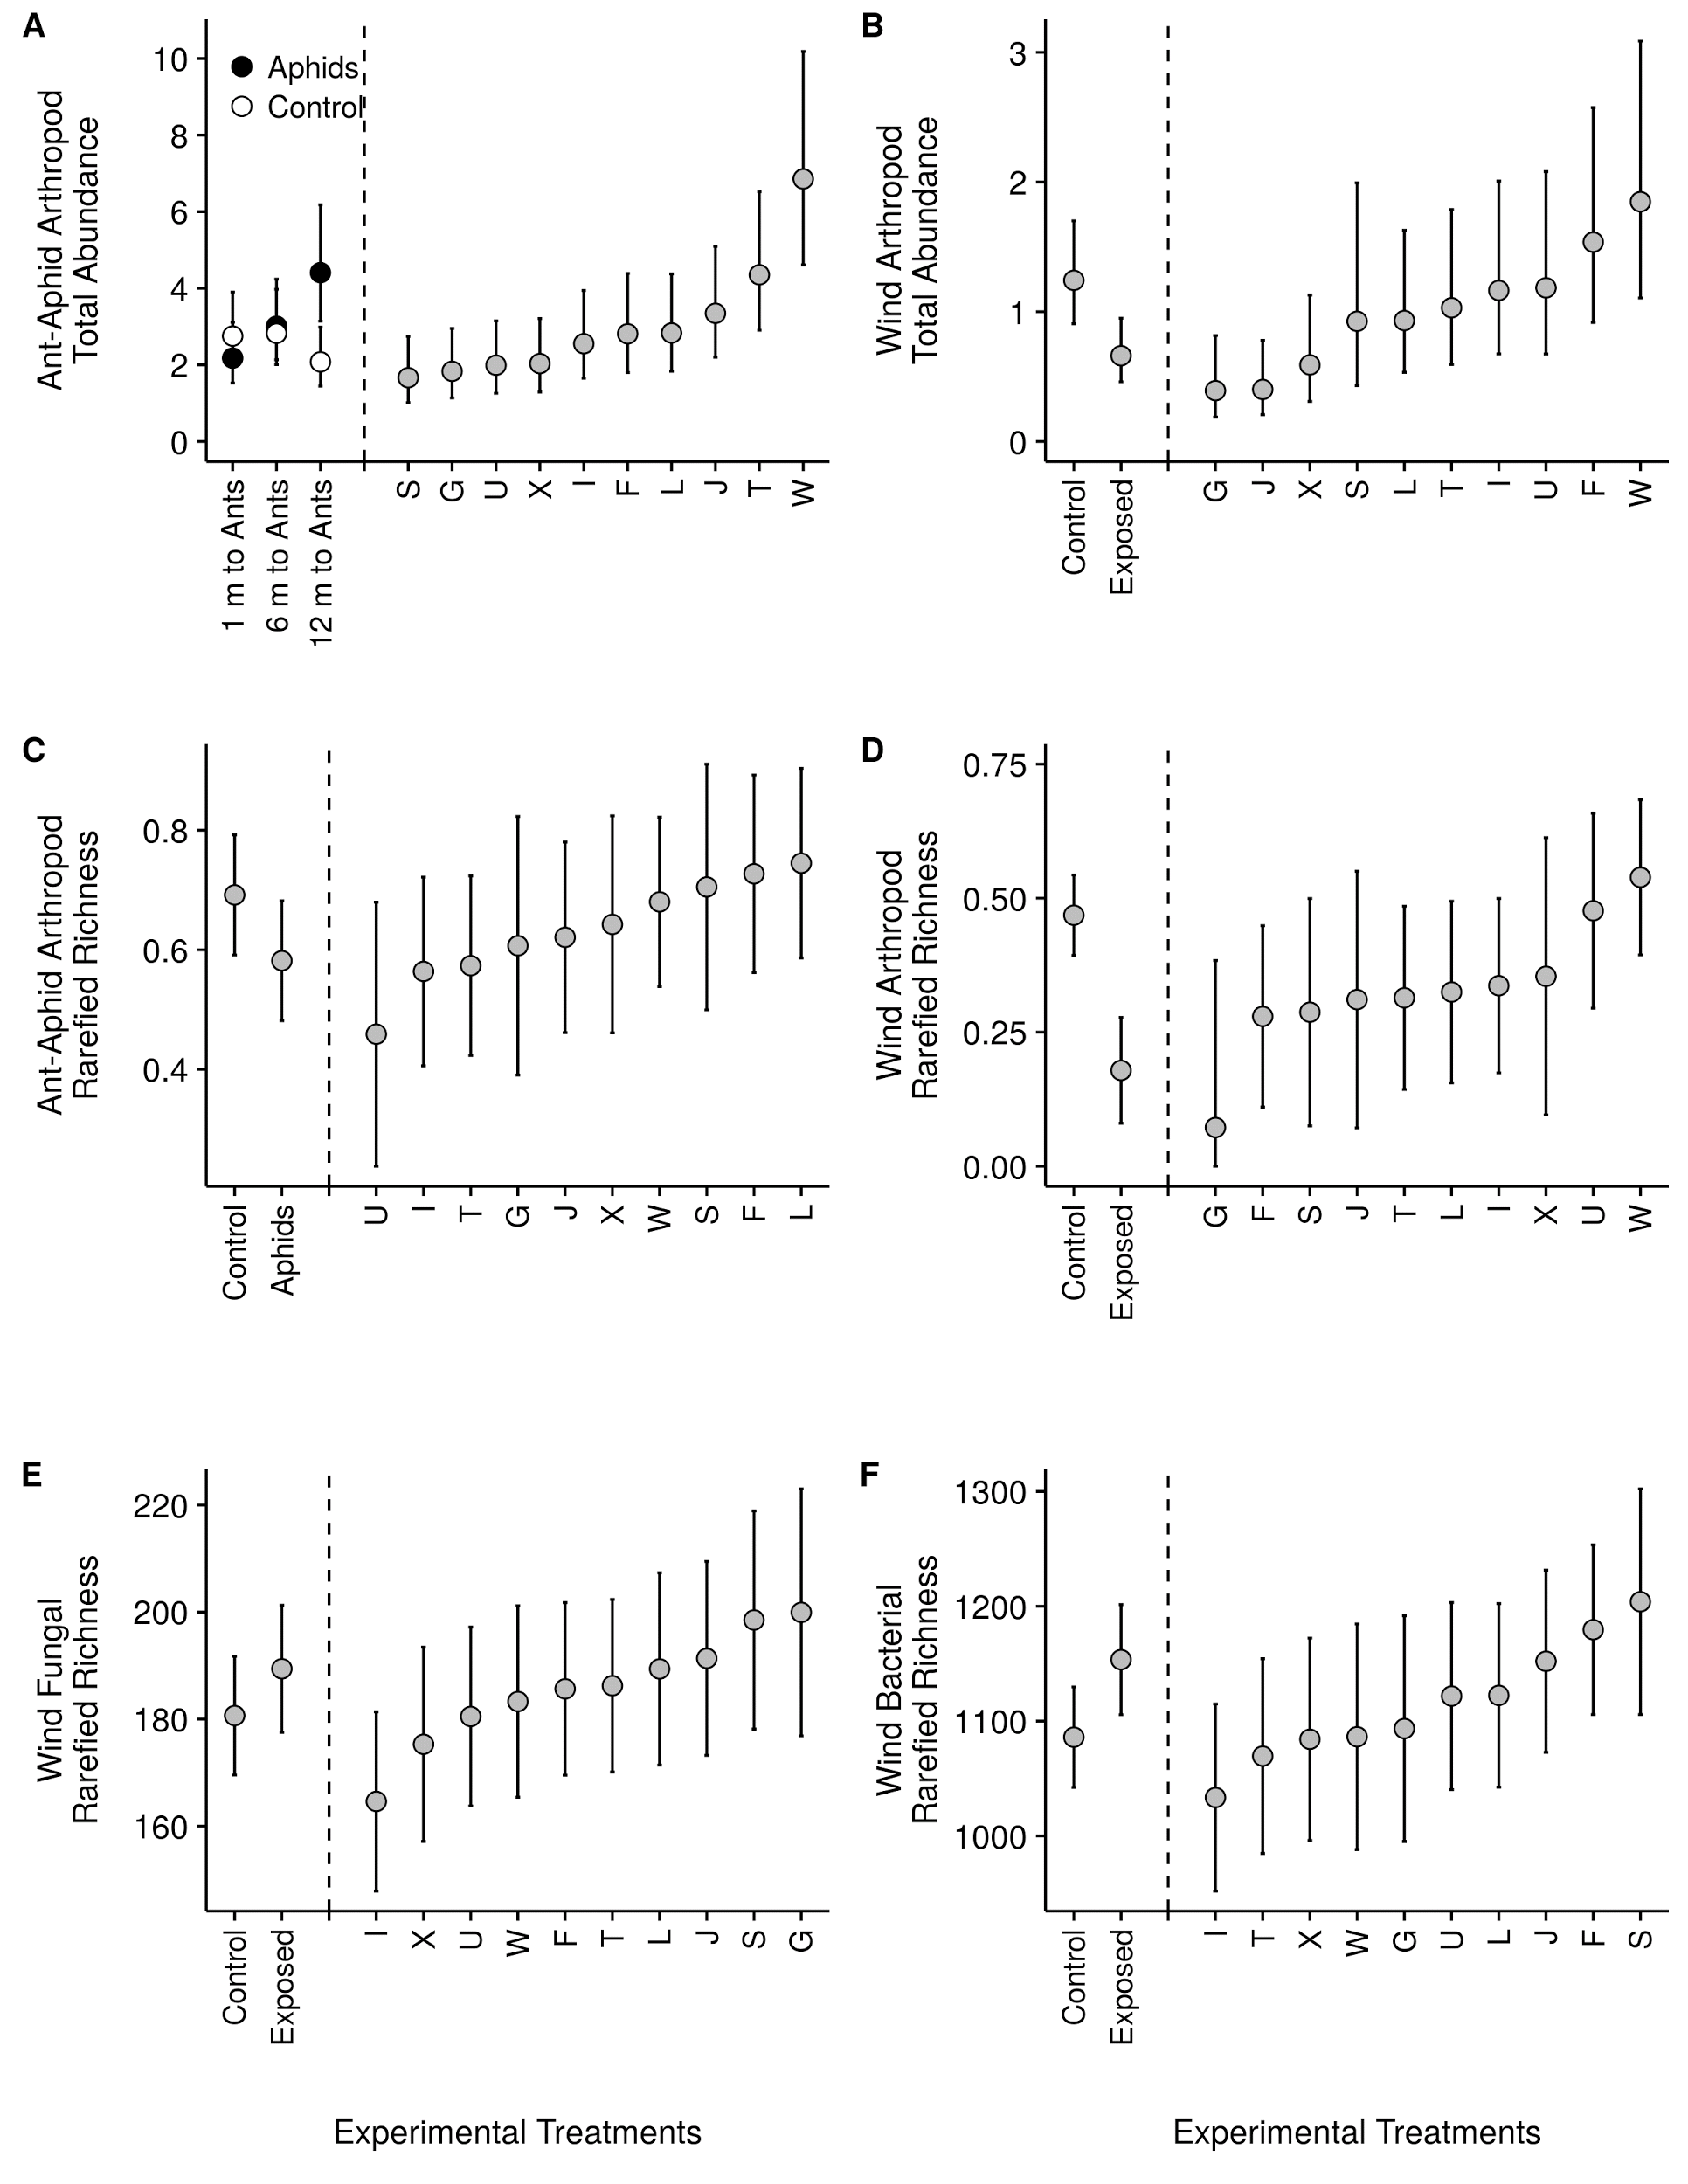
\includegraphics[scale = 0.16]{image03.png}
\caption{Effects of genetic variation within the willow
\textit{Salix hookeriana} as well as biotic (aphid additions and proximity
to ant mounds) and abiotic (wind exposure) factors on the structure of
above and belowground communities. Willow genotype had strong effects on
arthropod abundance in both the ant-aphid (A) and wind exposure (B)
experiments. In the ant-aphid experiment (A), arthropod abundance was
influenced by the addition of the aphid \textit{Aphis farinosa}, but only
at the furthest distance from mounds of the ant \textit{Formica
obscuripes}. In the wind experiment (B), wind exposure reduced arthropod
abundance. In contrast to arthropod abundance, willow genotype had weak
effects on arthropod rarefied richness in both the ant-aphid (C) and
wind exposure (D) experiments. In the ant-aphid experiment (C), the
addition of aphids reduced the probability of encountering a different
arthropod species (rarefied richness). In the wind experiment (D), wind
exposure dramatically reduced arthropod rarefied richness. Similar to
arthropod rarefied richness, willow genotype had weak effects on the
rarefied richness of rhizosphere fungi (E) and bacteria (F). While wind
exposure had a weak effect on fungal rarefied richness (E), we found
that wind exposed willows hosted a more diverse community of rhizosphere
bacteria (F). Points and error bars correspond to the response
variable's mean $\pm$ 95\% confidence interval. We calculated mean and confidence intervals based on the full models (Tables \ref{aaCommTrait},\ref{wComm}) using the \textit{effects} package in R.}
\label{Fig:GxEuni}
\end{figure}

\begin{figure}[h!]
\centering
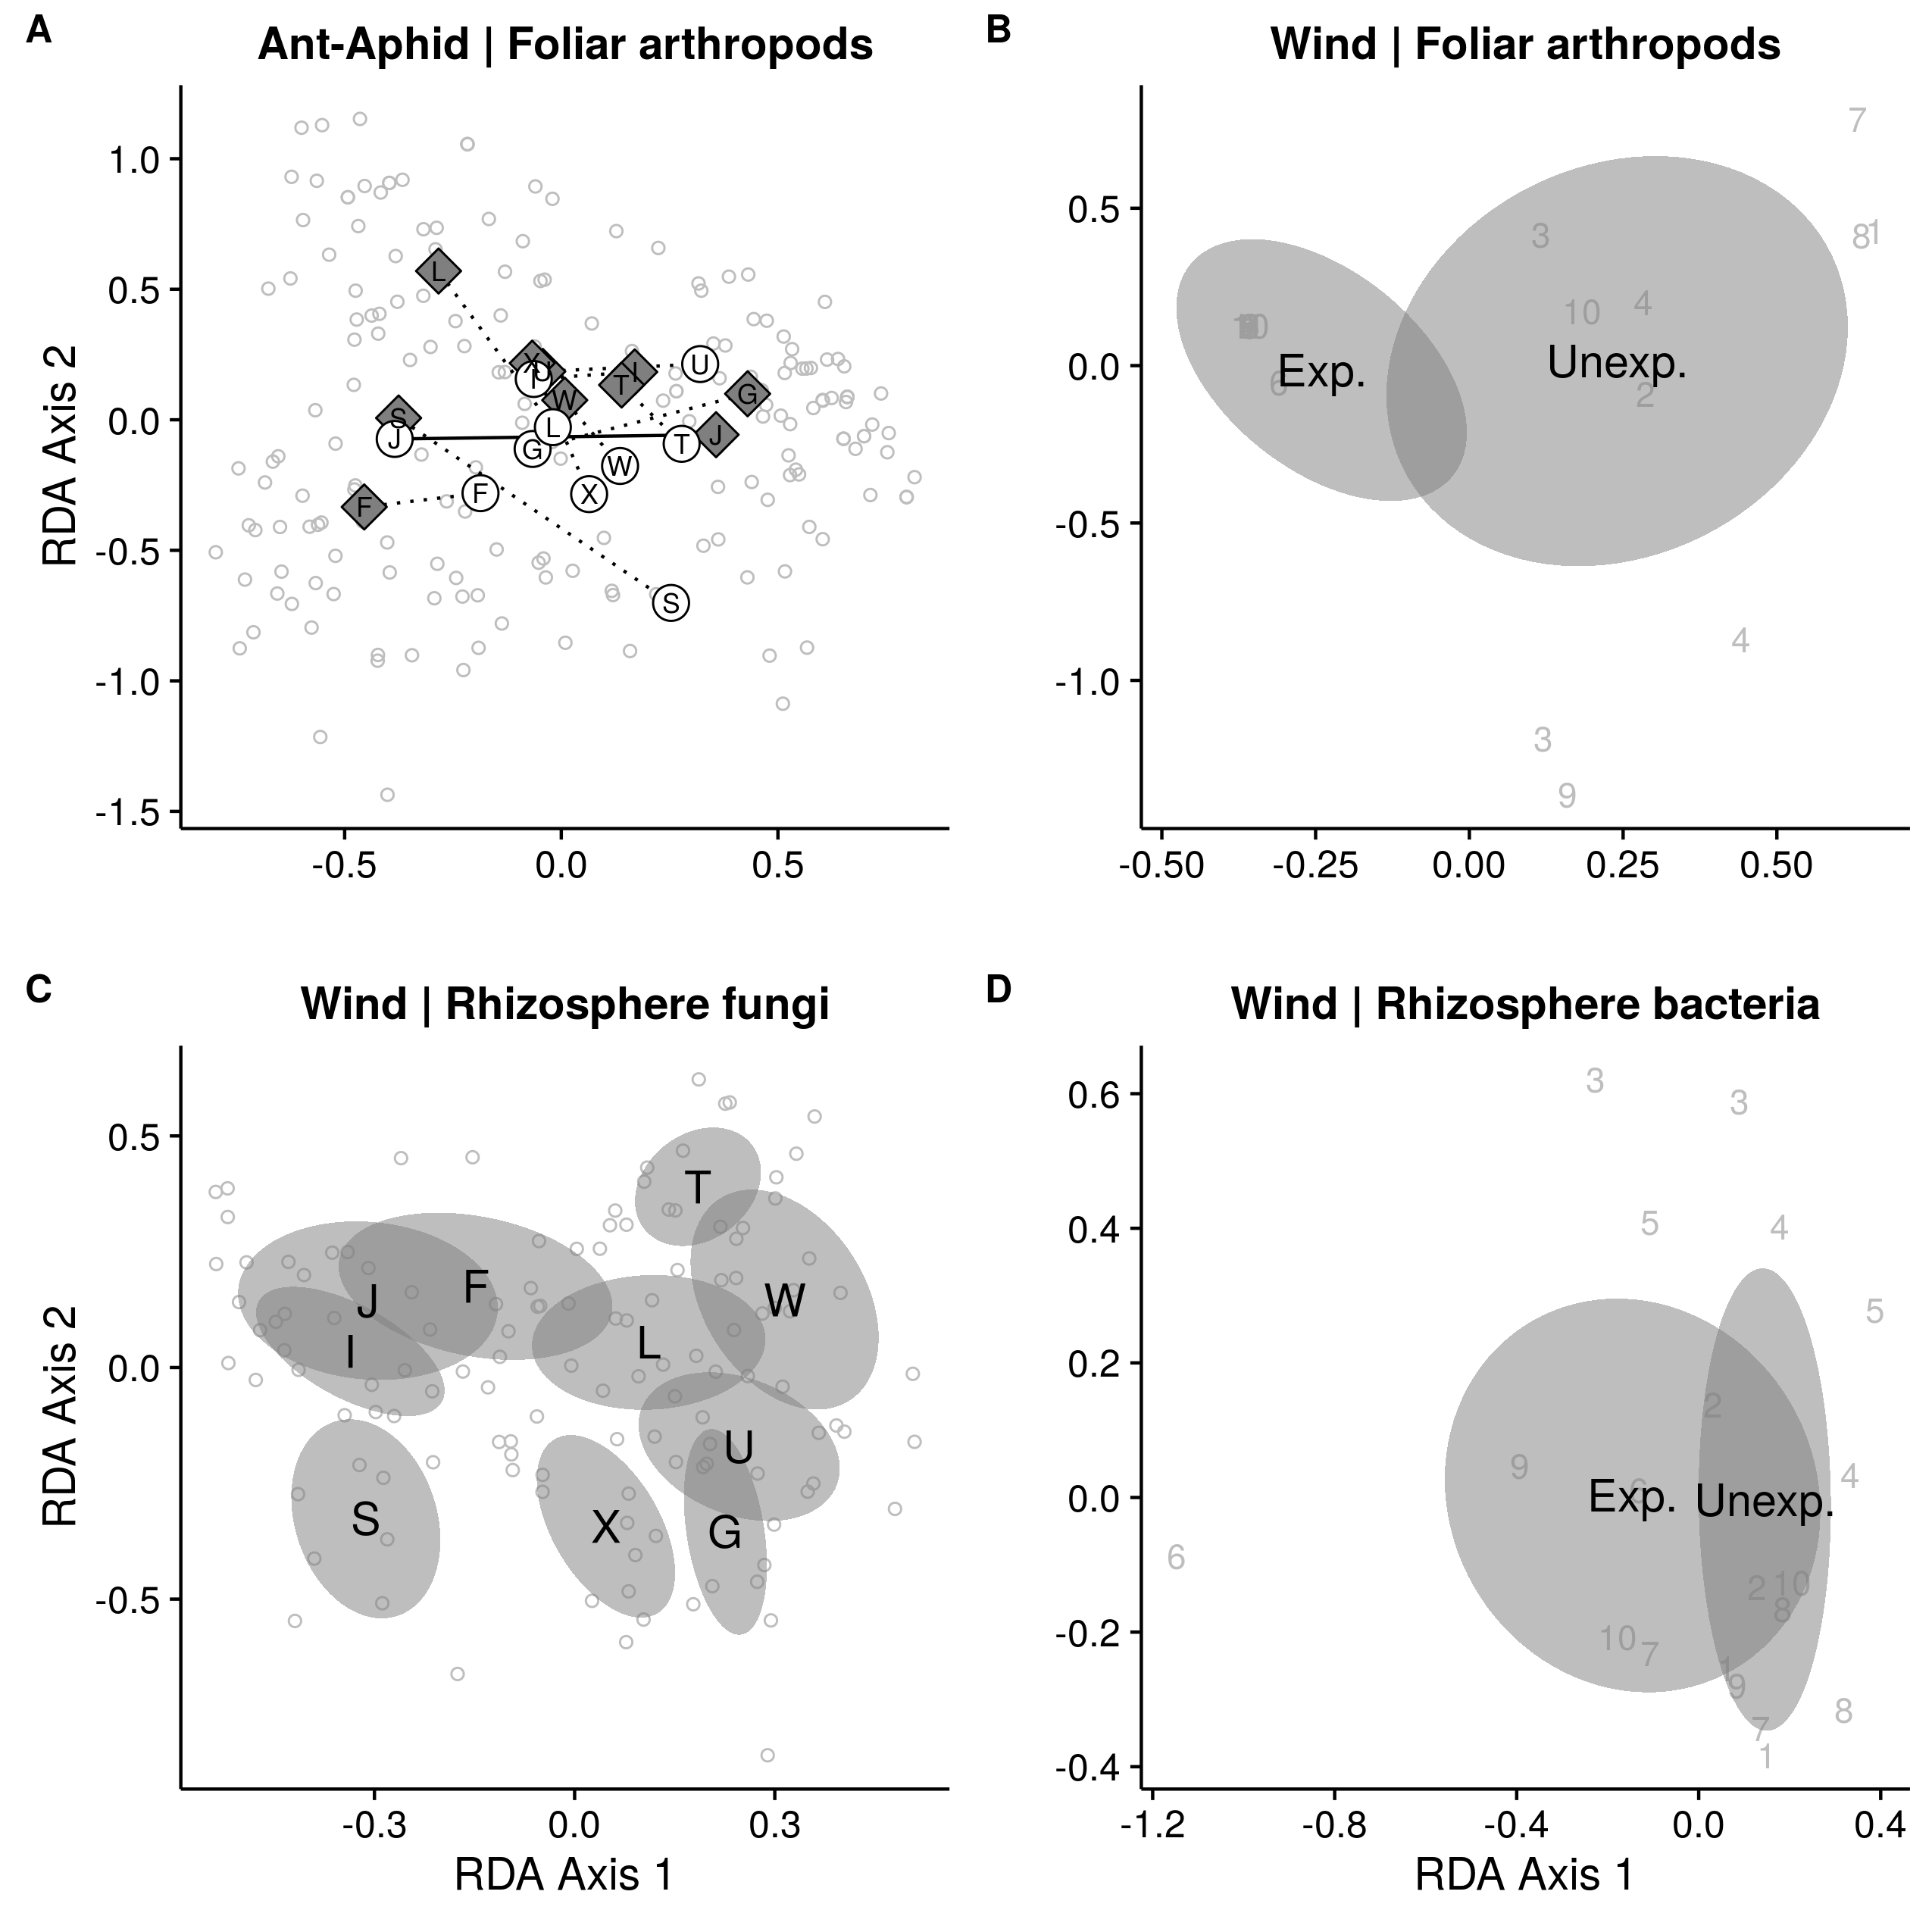
\includegraphics[scale = 0.65]{fig_2.png}
\caption{Effects of genetic variation within the willow
\emph{\textit{Salix hookeriana}} as well as biotic (aphid additions) and
abiotic (wind exposure) factors on the composition of above and
belowground communities. In the ant-aphid experiment (A), the addition
of the aphid \emph{Aphis farinosa} (grey diamonds) modified the
effect of willow genotype on the composition of the arthropod community.
This interaction between willow genotype and aphid treatment was solely
due to the differential effect of genotype J (solid line) on the
abundance of non-\emph{A. farinosa} aphids in the aphid treatment (Table \ref{aaGuild}).
For arthropods in the wind experiment (B), we found that wind exposure
had a strong effect on community composition in 2013 (but not 2012,
Table \ref{wComm}), with no clear effect of willow genotype. Belowground, we
found that willow genotype influenced the composition of rhizosphere
fungi (C), while the composition of rhizosphere bacteria was only influenced
by wind exposure (D). Black text and grey ellipses correspond to the
community centroid $\pm$ 95\% confidence interval. Grey numbers denote
blocks and each unique number is the community centroid for the plot
within each block. Grey circles mark the location of individual willow
communities in multivariate space. We calculated the locations of
centroids $\pm$ 95\% confidence interval and individual samples using
redundancy analysis on Hellinger-transformed community data.}
\label{Fig:GxEcomp}
\end{figure}

\begin{figure}[h!]
\centering
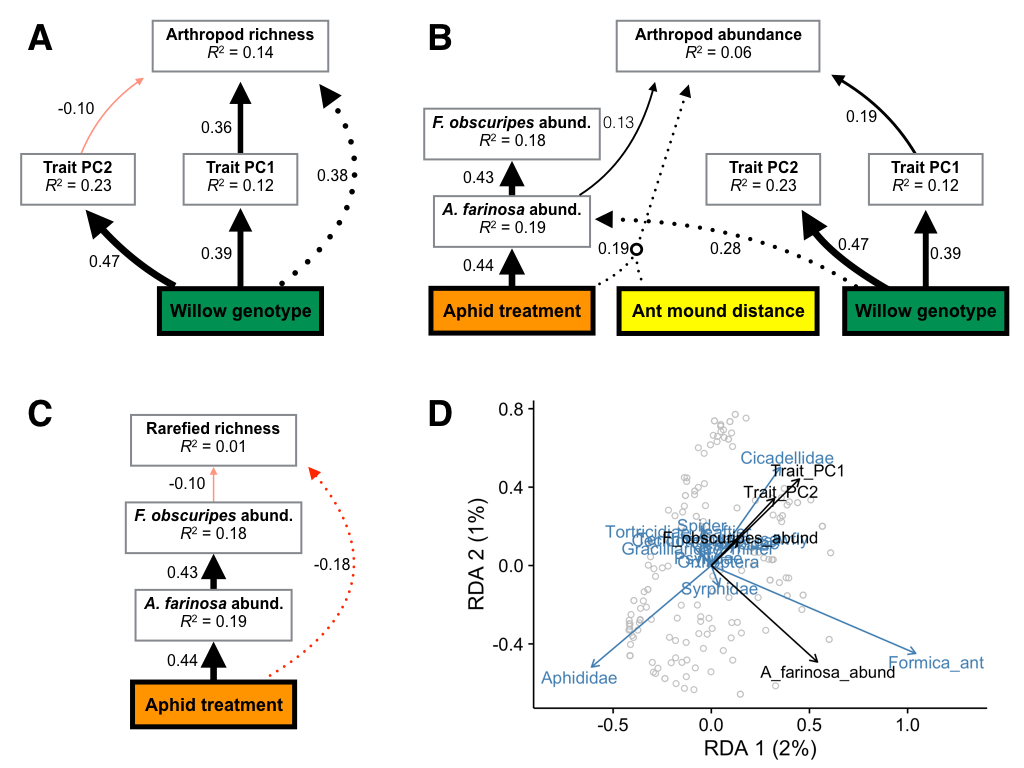
\includegraphics[scale = 0.45]{image04.png}
\caption{Statistical models of the processes mediating
arthropod community assembly in the ant-aphid experiment. Piecewise
structural equation models of arthropod richness (A), abundance (B), and
rarefied richness (C). Colored and white boxes represent exogenous and
endogenous variables, respectively. Solid, single-headed arrows
correspond to modeled pathways between predictor and response variables,
and may be either positive (black) or negative (red). For clarity,
we only plotted paths with standardized coefficients $>$
0.10, but marginally significant effects (0.05 $<$ P $<$ 0.10) are transparent. Numbers next to all arrows represent the standardized path
coefficient, which also corresponds to the thickness of arrows. (D)
Redundancy analysis illustrating the effect of plant traits (Trait PC1, PC2) and \textit{A. farinosa} abundance on the arthropod community (Hellinger-transformed = square root of proportional abundances of species found on each willow).
Black and blue arrows correspond to plant traits and species,
respectively, while grey dots represent the position of individual
willow communities.}
\label{aaSEM}
\end{figure}

\begin{figure}[h!]
\centering
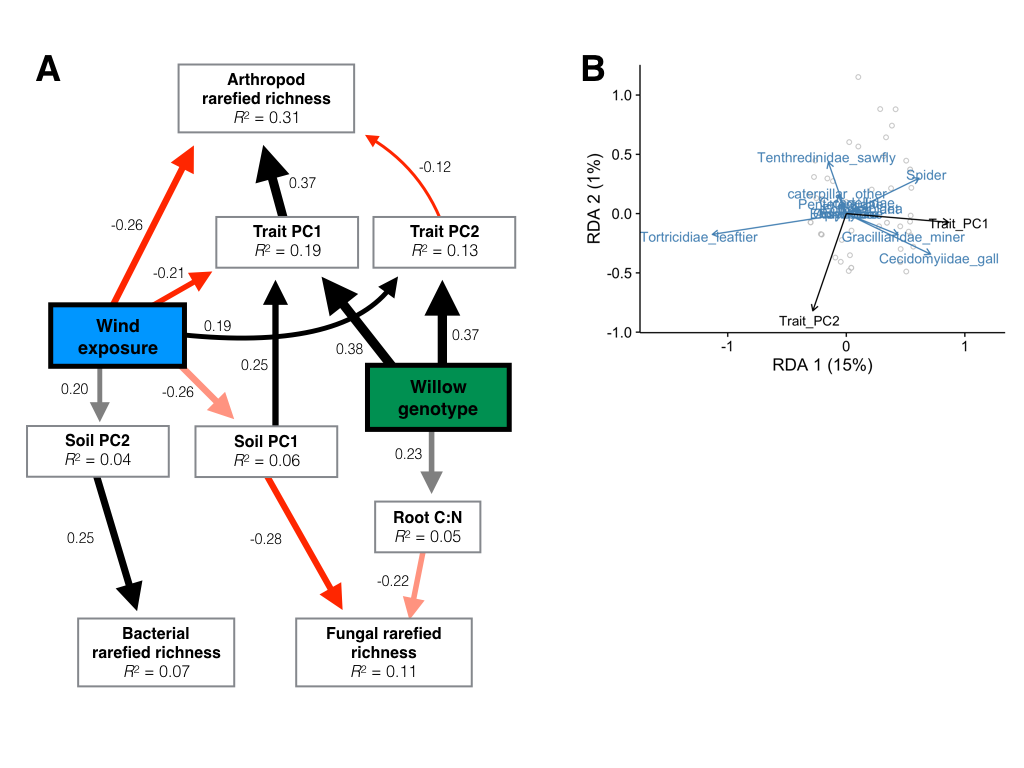
\includegraphics[scale = 0.45]{image05.png}
\caption{Statistical models of the processes mediating
community assembly in the wind experiment for 2013. (A) Piecewise
structural equation model of the rarefied richness of foliar arthropods
as well as root fungi and bacteria. Colored and white boxes represent
exogenous and endogenous variables, respectively. Solid, single-headed
arrows correspond to modeled pathways between predictor and response
variables, and may be either positive (black) or negative (red). For clarity,
we only plotted paths with standardized coefficients $>$
0.10, but marginally significant effects (0.05 $<$ P $<$ 0.10) are transparent. Numbers next to all arrows represent the standardized path
coefficient, which also corresponds to the thickness of arrows. (B)
Redundancy analysis illustrating the effect of plant traits (Trait PC1, PC2) on the arthropod community (Hellinger-transformed = square root of proportional abundances of species found on each willow).
Black and blue arrows correspond to plant traits and species,
respectively, while grey
dots represent the position of individual willow communities.}
\label{wSEM}
\end{figure}

%\subsection*{Online figure legends}

%\renewcommand{\thefigure}{A\arabic{figure}}
%\setcounter{figure}{0}

%\begin{figure}[h!]
%\includegraphics{jumps20m}
%\caption{\textit{A}, the quick red fox proceeding to jump 20~m straight 
%into the air over not one, but several lazy dogs. \textit{B}, the quick 
%red fox landing gracefully despite the skepticism of naysayers.}
%\label{Fig:Jumps}
%\end{figure}

%\begin{figure}[h!]
%\includegraphics{jumps-nr-okapi}
%\caption{The quicker the red fox jumps, the likelier it is to land near 
%an okapi. For further details, see \citet{LemKapEx07}.}
%\label{Fig:JumpsOk}
%\end{figure}

%\renewcommand{\thefigure}{B\arabic{figure}}
%\setcounter{figure}{0}

\end{document}

